% =============================================================================
% FAECO — 基于局部冲突诊断与保护式重布线的限时布线后门级面积回收方法（V4）
% 中文学术主稿（LuaLaTeX 编译）
% =============================================================================
\documentclass[twocolumn,10pt,fontset=windows]{ctexart}

% -----------------------------------------------------------------------------
% 字体
% -----------------------------------------------------------------------------
\setmainfont[Path=./fonts/,Extension=.ttf,UprightFont=times,BoldFont=timesbd,ItalicFont=timesi,BoldItalicFont=timesbi]{Times New Roman}
\setCJKmainfont[Path=./fonts/,Extension=.ttf,BoldFont=SimHei]{FZShuSong-Z01}
\setCJKsansfont[Path=./fonts/,Extension=.ttf]{SimHei}
\newCJKfontfamily\songfamily[Path=./fonts/,Extension=.ttf]{FZShuSong-Z01}
\newCJKfontfamily\fangfamily[Path=./fonts/,Extension=.ttf]{FZFangSong-Z02}
\newCJKfontfamily\heifamily[Path=./fonts/,Extension=.ttf]{SimHei}
\let\songti\songfamily\let\heiti\heifamily\let\fangsong\fangfamily

% -----------------------------------------------------------------------------
% 宏包
% -----------------------------------------------------------------------------
\usepackage{amsmath,amssymb}
\usepackage{newtxmath}
\usepackage{booktabs}
\usepackage{graphicx}
\usepackage{float}
\usepackage{array}
\usepackage[nocompress]{cite}
\usepackage[hidelinks]{hyperref}
\usepackage{xurl}
\usepackage{algorithm}
\usepackage{algpseudocode}
\floatname{algorithm}{算法}
\usepackage{multirow}
\usepackage{geometry}
\usepackage{placeins}
\usepackage{dblfloatfix}
\usepackage[noshrink,nospread]{flushend}

% -----------------------------------------------------------------------------
% 版面
% -----------------------------------------------------------------------------
\geometry{a4paper,left=2.0cm,right=2.0cm,top=2.1cm,bottom=2.1cm,columnsep=28pt}
\renewcommand{\eqref}[1]{\textup{（\ref{#1}）}}
\graphicspath{{../figures/}}
\setlength{\emergencystretch}{3em}
\Urlmuskip=0mu plus 3mu\relax
\raggedbottom
\setlength{\floatsep}{6pt plus 2pt minus 2pt}
\setlength{\textfloatsep}{8pt plus 2pt minus 2pt}
\setlength{\intextsep}{6pt plus 2pt minus 2pt}
\setlength{\dblfloatsep}{6pt plus 2pt minus 2pt}
\setlength{\dbltextfloatsep}{8pt plus 2pt minus 2pt}

% -----------------------------------------------------------------------------
% 标题层级
% -----------------------------------------------------------------------------
\ctexset{
  section = {format=\heiti\fontsize{11.5}{15}\selectfont, beforeskip=6pt, afterskip=4pt},
  subsection = {format=\heiti\fontsize{10.5}{14}\selectfont, beforeskip=5pt, afterskip=3pt},
  subsubsection = {format=\songti\fontsize{10}{13}\selectfont, beforeskip=4pt, afterskip=2pt}
}

% -----------------------------------------------------------------------------
% 图题/表题
% -----------------------------------------------------------------------------
\usepackage{caption}
\DeclareCaptionFont{songti}{\songti}
\DeclareCaptionFont{heiti}{\heiti}
\captionsetup[figure]{font={songti,small},labelfont={bf},skip=3pt}
\captionsetup[table]{font={heiti,small},labelfont={bf},skip=3pt}
\captionsetup{labelsep=space}

\begin{document}

\pagestyle{plain}

% ============================================================
% 中文首部：标题/作者/单位/摘要/关键词
% ============================================================
\twocolumn[
\vspace*{-0.25cm}
\begin{center}
{\heiti\zihao{3} FAECO：基于局部冲突诊断与保护式重布线的限时布线后门级面积回收方法}\par
\vspace{6pt}
{\fangsong\zihao{4} 佟亚龙、刘畅}\par
\vspace{4pt}
{\songti\fontsize{8}{12}\selectfont（国防科技大学计算机学院，长沙 410073）}\par\vspace{2pt}
{\songti\fontsize{8}{12}\selectfont E-mail：chancews@qq.com（通信作者）}\par
\vspace{6pt}
\end{center}
\begin{flushleft}
  {\heiti\fontsize{8.5}{13}\selectfont 摘\quad 要：}{\songti\fontsize{8.5}{13}\selectfont
  多工艺角时序收敛阶段因布线前寄生估算偏差普遍引入保守单元放大，遗留可观的面积与功耗冗余；详细布线完成后全芯片重布线会大范围扰动已收敛互连与时钟树，故物理实现流程广泛采用布线后门级工程变更（ECO）实施局部降尺寸回收。与同占位多阈值电压替换不同，跨物理占位降尺寸会改变引脚与障碍几何，与邻近已布线信号网产生瞬时金属冲突；若盲目放行周边邻网，耦合电容扰动又极易触发亚皮秒保持时间退化。针对上述物理耦合难题，本文提出有限时间预算下的布线后门级面积回收框架FAECO，核心耦合三项机制：（1）基于标准单元行高自适应缩放（$1.0\times H_{\mathrm{row}}$，无需人工工艺调参）的局部窗口化布线前设计规则检查（DRC）诊断，结合原地替换零位移与局部几何不变式精确归因冲突邻网集合，并锁定外围无冲突线网执行保护式局部重布线；（2）区分ECO合格解与绝对时序收敛状态的可调相对建立时间预算与三工艺角物理等价验证闭环；（3）有界乐观全池探针与保持时间反馈自适应微批次（含直连电容重排与确定性建立时间拒收去重）相结合的混合调度策略（Hybrid FAECO）。在130\,nm SKY130HD与7\,nm ASAP7双工艺四个主基准的720\,s墙钟配对实验中，局部窗口诊断在37组历史回放上与全块DRC的56处非零违例标记完全匹配（未观察到漏报），单次诊断提速3.04--16.69倍；在SKY130HD AES上，同一窗口后端下纯微批次FAECO回收98.8448\,\textmu m$^2$（为同后端单门与固定微批次的2.93倍），混合探针模式更在251\,s内兑现100\%候选池收益（197.6896\,\textmu m$^2$），而静态几何放行与原生功耗回收均为零；在7\,nm独立留出AES及绝对时序收敛UART基准上，FAECO均在完整物理与形式验证闭环下稳定交付功能标准单元面积与提取寄生功耗的同步下降。}
\par
\vspace{4pt}
{\heiti\fontsize{8.5}{13}\selectfont 关键词：}{\songti\fontsize{8.5}{13}\selectfont 布线后门级ECO，局部窗口化DRC诊断，保护式重布线，可调时序预算，混合自适应微批次调度}\par
\vspace{2pt}
{\songti\fontsize{8.5}{13}\selectfont 中图法分类号：TN402}\par
\vspace{3pt}
\end{flushleft}
]

% ============================================================
% 英文首部（元数据同步）
% ============================================================
\newcommand{\enTitle}{FAECO: Time-Budgeted Post-Route Gate Sizing with Localized Conflict Diagnosis and Protected Rerouting}
\newcommand{\enAuthor}{Tong Yalong, Liu Chang}
\newcommand{\enAffil}{(College of Computer Science and Technology, National University of Defense Technology, Changsha 410073)}
\newcommand{\enAbstract}{%
  Conservative cell upsizing during pre-route timing closure leaves substantial area and power redundancy, yet full place-and-route after detailed routing perturbs converged interconnects and clock trees. Post-route cross-footprint gate downsizing recovers this redundancy surgically, but alters cell widths and pin access geometries, inducing immediate shorts with adjacent routed wires; conversely, over-releasing non-conflicting neighbors perturbs coupling capacitances and triggers sub-picosecond hold regressions. We present FAECO, a time-budgeted post-route gate-level ECO framework centered on localized conflict diagnosis and protected rerouting. FAECO integrates: (1) row-height-adaptive ($1.0\times H_{\mathrm{row}}$) local-windowed pre-route DRC diagnosis with formal geometric coverage bounds over pin-access layers to attribute conflicting neighbor nets while locking non-conflicting routes; (2) an adjustable relative setup-loss budget distinguishing ECO-qualified from timing-closed states under multi-corner STA, whole-block DRC, antenna, and sequential equivalence checking (SEC); and (3) a hybrid scheduler coupling a bounded optimistic full-pool probe with hold-feedback adaptive microbatching and deterministic setup-rejection deduplication. Across four dual-PDK benchmarks (130\,nm SKY130HD and 7\,nm ASAP7) under 720\,s wall-clock limits, windowed diagnosis matches all 56/56 non-zero full-block markers across 37 historical replays with $3.04\times$--$16.69\times$ speedup; under the identical windowed backend on SKY130HD AES, microbatch FAECO achieves 98.8448\,\textmu m$^2$ ($2.93\times$ over matched single-gate and fixed-batch baselines) and Hybrid FAECO captures 100\% of the pool (197.6896\,\textmu m$^2$) in 251\,s, while preserving full cross-design delivery across all four benchmarks and an additional timing-closed 7\,nm benchmark.%
}
\newcommand{\enKeywords}{post-route gate-level ECO, localized DRC conflict diagnosis, protected rerouting, adjustable timing budget, hybrid adaptive microbatch scheduling}

% ============================================================
% §1 引言
% ============================================================
\section{引言}

在现代超大规模集成电路与片上系统（system-on-chip，SoC）的物理实现流程中，性能、功耗与面积（power, performance, and area，PPA）的协同优化贯穿逻辑综合、布局、时钟树综合（clock tree synthesis，CTS）与详细布线的全周期\cite{chinnery2002closing,openroad}。然而，布线前阶段所依赖的线载模型或全局布线寄生估算与详细布线后的实际互连电阻电容之间存在结构性偏差，加之电路须同时满足快角（FF）、典型角（TT）与慢角（SS）等多工艺角时序约束，物理综合与时序修复引擎（如OpenROAD Resizer\cite{openroad}）在修复建立时间与电气违例时普遍施加保守裕量，对非关键路径引入过度的单元放大。本文对八个ISCAS89基准的逐门诊断表明，时序修复引入的107处单元放大中，有74处（69\%）在单独回退后于报告精度内不恶化最差建立时间负松弛（worst negative slack，WNS）。此类冗余单元持续增加有效功能单元面积、栅极电容与亚阈值漏电。

在物理设计后期阶段，若为回收上述冗余而重跑全芯片布局布线（place-and-route，P\&R），不仅计算耗时漫长，而且会大范围改写数以万计条已布线信号网的几何拓扑与串扰耦合环境，破坏既有的建立/保持时间平衡与时钟偏斜，迫使全芯片重新开展多角时序、物理规则与形式等价验证。因此，工业与开源物理实现流程均在详细布线冻结后引入\textbf{布线后门级工程变更（engineering change order，ECO）}环节\cite{lee2012eco,fatemi2019sizer,cheng2023dagsizer}，在严格锁定外围已布线版图的前提下定点回收非关键单元。本文的研究定位聚焦于\textbf{有限时间预算下的布线后ECO验证效率与低扰动面积回收}，而非替代前期全芯片PPA综合。

与保持标准单元物理占位不变（same-footprint）的多阈值电压（$V_t$）或沟道长度替换不同\cite{cheng2023dagsizer}，\textbf{跨物理占位的降驱动尺寸替换（cross-footprint downsizing）}在布线后阶段面临更棘手的物理耦合问题。即便采用不移动任何相邻单元的原地单元替换（in-place cell substitution），缩小单元驱动强度仍会改变单元宽度、内部引脚接入位置及底层金属障碍物轮廓，致使原本合法穿越该区域的邻近信号网与新单元产生瞬时金属短路或最小间距违例。因而，布线后降尺寸必须与保护式局部详细重布线、基于详细布线的寄生参数提取（parasitic extraction，RCX）、三工艺角静态时序分析（static timing analysis，STA）、独立全块DRC、天线检查及全网表顺序等价性检查（sequential equivalence checking，SEC）耦合为完整的在线验证闭环\cite{tritonroutewxl,yosys}。

将上述完整物理验证闭环置于有限墙钟预算（anytime wall-clock budget）约束下，凸显出三项相互制约的关键问题：
\begin{enumerate}
\item \textbf{邻线冲突归因与亚皮秒保持时间敏感性。} 若仅重布被替换单元的直连信号网，残留在新轮廓附近的旧邻线违例将导致详细布线难以收敛并触发整轮复修；反之，若采用静态几何邻近规则预先放行邻网（如释放与目标单元边界接触的全部底层信号线），多余放行的无冲突保护网在重布后改变耦合电容，极易在亚皮秒级相对保持时间（hold）约束下导致原本合格的候选被拒收。
\item \textbf{全块布线前DRC验证的尺度扩展瓶颈。} 在原地替换并擦除直连旧线后执行全块布线前DRC虽可精确归因冲突邻网，但单次扫描耗时随版图面积近似线性增长——在130\,nm万门级模块上约14\,s，在7\,nm 22.8k实例模块上增至38--45\,s，在低冲突大规模先进工艺版图上成为限时预算的主要固定开销。
\item \textbf{离线大批次提交的跨设计脆弱性与在线小批次吞吐的权衡。} 经典拉格朗日松弛（Lagrangian relaxation，LR）或单角内置回收启发式基于冻结的标准寄生交换格式（SPEF）一次性提交大批次候选：当设计多角裕量充足且配备保护后端时可迅速兑现高额面积，但一旦遭遇局部拥塞或跨角时序悬崖便整体失效（零交付）；反之，纯逐门或固定小微批次虽更稳健，却在全池可一次交付的场景下受限于串行验证轮数。
\end{enumerate}

针对上述问题，本文提出基于局部冲突诊断与保护式重布线的限时布线后门级面积回收框架\textbf{FAECO}。本文的核心贡献概括如下：
\begin{enumerate}
\item \textbf{行高自适应$1.0\times H_{\mathrm{row}}$局部窗口化布线前DRC冲突诊断与理论边界。} 以集合对称差与闵可夫斯基膨胀形式化证明局部窗口对引脚层局部短路与成对间距规则的几何覆盖完备性（命题~1），并解析SKY130HD（130\,nm）与ASAP7（7\,nm）真实工艺技术LEF规则逐层核验作用半径与行高$H_{\mathrm{row}}$的覆盖关系。无需人工工艺调参，机制自动将窗口半径缩放为$1.0\times H_{\mathrm{row}}$，在37组历史回放中与全块DRC的56处非零违例标记完全匹配（未观察到漏报），单次诊断提速3.04--16.69倍；受控变量消融表明，精准锁定冲突邻网避免了过度放行诱发的$-10.48$\,ps慢角保持时间退化，构成跨占位布线后ECO的核心物理使能机制。
\item \textbf{区分ECO合格与绝对收敛的限时验证模型及多维评测体系。} 严格界定\textbf{ECO合格解（ECO-qualified）}与\textbf{绝对时序收敛（Timing-closed）}两类状态，建立可调相对建立时间预算、三工艺角Hold WNS非负非退化、零新增电气违例、独立全块DRC/天线清零及全网表SEC验证协议；配套提出候选池捕获率、相对基线增益、建立时间预算利用率、时间平均随时合格回收（normalized Anytime AUC）与提取寄生功耗五维评测指标。
\item \textbf{混合自适应调度（Hybrid FAECO）、同窗口组件消融与跨工艺实证。} 将有界乐观全池探针与保持时间反馈自适应微批次（含Hold暂缓、直连电容代理重排与确定性建立时间拒收去重）耦合：探针通过时直接交付100\%候选池收益，受阻时在子预算内截断并无损回退至微批次闭环。在130\,nm与7\,nm双工艺四个主基准及新增绝对时序收敛基准上的配对实验表明：同一窗口后端下直连电容重排在SKY130HD AES上独立贡献2.93倍终态面积增益（98.8448对33.7824\,\textmu m$^2$），Hybrid FAECO在251\,s内进一步兑现197.6896\,\textmu m$^2$（100\%候选池）且在其余3个基准上零面积损失回退，全部基准均交付0\,DRC、0天线、SEC全证且提取寄生功耗同步下降的ECO合格版图。
\end{enumerate}

% ============================================================
% §2 相关工作与对比定位
% ============================================================
\section{相关工作与对比定位}

\subsection{门尺寸优化、拉格朗日松弛与布线后功耗回收}

离散门尺寸调整与阈值电压分配是物理设计中平衡时序、面积与功耗的经典组合优化问题\cite{chinnery2002closing,ozdal2012ispd,hu2013ispd}。以拉格朗日松弛为代表的数学规划范式\cite{chen1999fast,flach2014effective}通过次梯度迭代更新乘子并求解局部加权代价最小化，在固定寄生假设下具有较高求解速度；Mangiras等\cite{timing_budget}利用任务图并行化进一步提升了大规模电路的尺寸迭代吞吐。Trident~2.0\cite{trident2}将启发式尺寸搜索直接耦合至签核级计时器以消除延迟模型偏差，但其优化循环仍基于固定寄生，未闭环布线后详细重布线与寄生重提取。

针对流片前的布线后功耗回收，现有工作主要沿两类路径展开。第一类聚焦保持单元物理占位不变的同尺寸替换：DAGSizer\cite{cheng2023dagsizer}采用有向图卷积网络预测多阈值电压与多沟道长度替换后的路径延迟偏移以削减定时器调用；Sizer\cite{fatemi2019sizer}面向工业多角多模式（MCMM）环境改进了灵敏度驱动回收启发式，但其后端实现依赖商业物理闭环。第二类如开源工具OpenROAD内置功耗回收引擎\cite{openroad}，在单一典型角与冻结寄生下依据正松弛门限执行降尺寸，难以预见重布线后的跨角建立/保持时间偏移及天线效应。Lee与Gupta\cite{lee2012eco}从线性规划视角建模了后期工艺漂移下的增量门尺寸ECO代价，但未涉及密集互连下的动态邻网冲突归因与有限墙钟闭环。

\subsection{局部物理ECO、布线协同修复与学习辅助优化}

当单元修改引起引脚几何与金属障碍物变化时，局部布局与详细布线的协同收敛决定ECO成败。TritonRoute-WXL\cite{tritonroutewxl}在开源详细布线器中集成增量DRC引擎，为快速检测局部金属短路、间距与过孔违例提供了底层支撑。CoRe-ECO\cite{coreeco}通过整数线性规划联合求解局部详细布局、详细布线与单元选型以消除既有引脚访问违例；面向7\,nm以下节点，SLO-ECO\cite{sloeco2024}将单线开路（single-line-open）图案热点纳入局部布线与布局协同优化。上述工作聚焦修复既有制造热点，未面向降尺寸面积回收主动诱发的邻网冲突进行候选组合调度与多角时序权衡。

近年来，强化学习、图神经网络与算法进化亦被引入物理综合与局部逻辑重构，包括OpenPhySyn\cite{openphysyn2020}、RL-Sizer\cite{rlsizer2021}、RL-CCD\cite{rlccd2023}、基于局部物理上下文的逻辑重映射\cite{pcr2026}、面向布局后逻辑重构的E-Layout\cite{elayout2026}以及目标驱动物理设计算法进化框架GoalEvolve\cite{goalevolve2026}。此类研究多作用于布局阶段或全局布线寄生估算层面，尚未面向已冻结详细布线版图在严格墙钟预算内闭环跨占位降尺寸、局部窗口冲突归因、保护式重布线与全网表等价性验证。表~\ref{tab:related_work}归纳了相关代表性工作与FAECO的方法论差异。

\begin{table*}[t]
\centering
\caption{代表性门尺寸优化、布线后回收与局部物理ECO方法对比}
\label{tab:related_work}
\scriptsize\setlength{\tabcolsep}{3.5pt}
\resizebox{\textwidth}{!}{%
\begin{tabular}{llllll}
\toprule
\textbf{方法} & \textbf{阶段与换门类型} & \textbf{优化目标} & \textbf{物理与寄生反馈} & \textbf{冲突处理与验证闭环} & \textbf{评测范式} \\
\midrule
Lee \& Gupta\cite{lee2012eco} & 后期增量尺寸调整 & ECO代价与时序约束 & 静态线性化延迟模型 & 无详细重布与邻网归因 & 离线单次 \\
Flach LR\cite{flach2014effective} & 离线全网门尺寸/$V_t$ & 面积/漏电最小化 & 冻结寄生与拉格朗日乘子 & 离线提交，无布线后多角闭环 & 离线单次 \\
Trident~2.0\cite{trident2} & 离散尺寸与$V_t$分配 & 漏电功耗、运行时间 & 签核计时器（固定寄生） & 时序/电气约束，无详细重布 & 离线单次 \\
Sizer\cite{fatemi2019sizer} & 工业布线后灵敏度回收 & 漏电与总功耗 & 工业MCMM时序与电气 & 商业后端，无跨占位冲突归因 & 单次运行 \\
CoRe-ECO\cite{coreeco} & 布线后局部DP/DR协同 & 引脚访问违例、线长 & 局部布局/布线联合求解 & 面向既有违例，不做面积回收 & 单次修复 \\
DAGSizer\cite{cheng2023dagsizer} & 同占位多$V_t$/沟长替换 & 漏电回收、预测精度 & 图神经网络与定时器标注 & 同占位免重布，不处理跨尺寸 & 离线推理 \\
SLO-ECO\cite{sloeco2024} & 7\,nm以下局部DP/DR & 单线开路与DRC清零 & 局部详细布线迭代优化 & 面向制造热点，不做面积回收 & 单次修复 \\
OpenROAD原生\cite{openroad} & 内置功耗回收引擎 & 非关键路径降尺寸 & 单角冻结寄生启发式 & 全片重布无保护，易多角违例 & 单次运行 \\
\textbf{FAECO（本文）} & \textbf{布线后跨占位降尺寸} & \textbf{限时合格面积与功耗} & \textbf{局部重布+提取RCX+三工艺角STA} & \textbf{$1.0H_{\mathrm{row}}$窗口归因+全块DRC/SEC} & \textbf{720\,s配对} \\
\bottomrule
\end{tabular}%
}
\end{table*}

% ============================================================
% §3 问题形式化与规范化评测体系
% ============================================================
\section{问题形式化与规范化评测体系}

\subsection{冻结参考状态界定、可调预算与ECO验证约束}

设已完成详细布线并通过零违例基线验证的冻结参考版图为$R$，包含完整的物理版图数据库、门级网表$N_R$、原始时序约束文件（SDC）及基于详细布线提取的寄生参数网络。记$A_R$为参考设计中\textbf{功能标准单元总面积}（不含物理填充与阱接触单元）。在三工艺角集合$\mathcal{V}=\{\mathrm{FF}, \mathrm{TT}, \mathrm{SS}\}$上，各角共用同一次详细布线后提取的名义寄生参数网络并分别加载对应工艺角标准单元时序库，以$W_v(N)$、$T_v(N)$和$H_v(N)$表示门级网表$N$在视图$v\in\mathcal{V}$下的建立时间WNS、建立时间总负松弛（TNS）以及保持时间WNS（正值表示余量充足，负值表示违例），并记参考时钟周期为$P_{\mathrm{clk}}$。

为避免将满足相对ECO约束与绝对时序收敛混为一谈，本文显式区分两类设计状态：
\begin{itemize}
\item \textbf{ECO合格状态（ECO-qualified）：} 候选交付版图$F(S)$相对冻结参考$R$满足下述式~\eqref{eq:obj}全部相对建立时间预算、多角Hold WNS非负且非退化、零新增电气违例、独立全块DRC清零、零天线违例及全网表SEC验证要求；该定义适用于包含残留建立时间负松弛的真实开源综合/布线起点。
\item \textbf{绝对时序收敛状态（Timing-closed）：} 在满足ECO合格状态的全部物理与形式约束基础上，进一步满足所有工艺角上的绝对建立时间与保持时间均非负，即$\forall v\in\mathcal{V},\; W_v(F)\ge 0$且$H_v(F)\ge 0$。
\end{itemize}

布线后限时门级面积回收问题形式化为：在给定严格墙钟预算$\tau_{\max}$（默认$\tau_{\max}=720$\,s，涵盖公共预筛、前沿排序、冲突诊断、局部重布、寄生提取、三工艺角STA、物理与形式验证及失败尝试的全部时间消耗）内，求解互异实例的兼容单元降尺寸替换集合$S=\{(g_1\to m_1), \dots, (g_k\to m_k)\}$，使交付版图$F(S)$最大化合格功能标准单元面积回收：
\begin{equation}
\label{eq:obj}
\begin{aligned}
\max_{S}\quad & \Delta A(S) = A_R - A\bigl(F(S)\bigr) \\
\text{s.t.}\quad & W_v\bigl(F(S)\bigr) \ge W_v(R) - B_W - \varepsilon, \quad \forall v\in\mathcal{V}, \\
                 & T_v\bigl(F(S)\bigr) \ge T_v(R) - B_{T,v} - \varepsilon, \quad \forall v\in\mathcal{V}, \\
                 & H_v\bigl(F(S)\bigr) \ge \max\bigl(0,\; H_v(R) - \varepsilon_h\bigr), \quad \forall v\in\mathcal{V}, \\
                 & \mathrm{ElecNew}\bigl(F(S)\bigr)=0,\quad \mathrm{DRC}_{\mathrm{full}}\bigl(F(S)\bigr)=0, \\
                 & \mathrm{Ant}\bigl(F(S)\bigr)=0,\quad \mathrm{SEC}\bigl(N_R, N_{F(S)}\bigr)=\mathrm{proven}, \\
                 & t_{\mathrm{complete}}(S) \le \tau_{\max}.
\end{aligned}
\end{equation}

其中，$B_W$为用户可调的建立时间WNS相对损失预算：在双工艺主实验中统一取$B_W = 0.01 P_{\mathrm{clk}}$以保持跨工艺频率尺度一致，在固定绝对预算扩展实验中取$B_W = 10$\,ps。各角建立时间TNS损失上限取$B_{T,v} = \max\bigl(0.10 P_{\mathrm{clk}},\, 0.01|T_v(R)|\bigr)$。建立时间与保持时间的数值比较容差均取$\varepsilon = \varepsilon_h = 0.001$\,ps（1\,fs）；需要明确指出，式~\eqref{eq:obj}约束的是三工艺角\textbf{Hold WNS非退化}而非逐路径保持时间单调性，且基于OpenROAD、OpenRCX与OpenSTA的完整验证闭环定位于开源ECO物理验证，不等同于商业晶圆厂终检签核（第~\ref{sec:boxed_eval}节进一步检验了重复RCX/STA的数值确定性与$\varepsilon_h$容差敏感性）。物理与形式验证要求零新增最大转换时间/最大电容电气违例、恢复完整布线态后的独立全块$\mathrm{DRC}_{\mathrm{full}}=0$、零天线违例以及全网表两态SEC零未证点。

\subsection{多维规范化随时可交付评测指标}

在固定芯片外框（die/core）的万门级布线后版图上，720\,s内经完整物理验证闭环回收的功能标准单元面积通常占总功能单元面积的$0.05\%$--$1.90\%$（标准单元面积下降用于释放局部布线资源与降低电容功耗，不直接等同于芯片制造外框缩小）。为全面刻画限时ECO的验证效率与空间兑现率，本文报告五项正交指标：
\begin{enumerate}
\item \textbf{候选池面积捕获率：} 设公共预筛生成$K$项\textbf{互异实例}的兼容候选池$\mathcal{P}$（主实验$K=18$，每实例至多包含一项替换，因而静态面积和$\Delta A_{\mathrm{pool}} = \sum_{i\in\mathcal{P}}\Delta A_i$构成严格可同时实现的面积上界），定义捕获率$\rho_{\mathrm{pool}} = \Delta A(S^*) / \Delta A_{\mathrm{pool}} \times 100\%$。该指标衡量在截断候选池内的兑现效率，与功能标准单元总面积降幅并列报告。
\item \textbf{相对基线增益倍率与共同目标首达提速：} 在相同冻结参考、候选池、后端模式与预算下，报告相对竞争基线的合格面积倍率及首次达到同一实际合格面积的墙钟提前量$\Delta t$（s）。
\item \textbf{建立时间预算利用率：} 定义$\eta_W = \max_{v\in\mathcal{V}}\max\bigl(0,\, W_v(R)-W_v(F)\bigr)/B_W \times 100\%$，量化对允许建立时间裕量的实际消耗。
\item \textbf{时间平均随时合格回收（normalized Anytime AUC）：} 记$a(t)$为策略在时刻$t\in[0,\tau_{\max}]$前已通过完整验证闭环的最大累计回收面积，定义时间归一化的平均随时回收：
\begin{equation}
\label{eq:auc}
\overline{A}_{[0,\tau_{\max}]} = \frac{1}{\tau_{\max}} \int_{0}^{\tau_{\max}} a(t)\,\mathrm{d}t.
\end{equation}
\item \textbf{提取寄生功耗联动收益：} 在典型角TT与详细布线提取寄生下，以统一开关活动度度量已交付合格端点相对参考$R$的总功耗、组合逻辑功耗与静态漏电变化。
\end{enumerate}

% ============================================================
% §4 FAECO 方法设计
% ============================================================
\section{FAECO 方法设计}

FAECO的整体方法架构如图~\ref{fig:arch}所示，由冻结已布线版图与兼容候选池构造、混合自适应调度（有界乐观全池探针与保持时间反馈自适应微批次）、行高自适应局部窗口化DRC冲突诊断与保护式局部重布线、以及三工艺角时序与物理等价验证构成闭环。系统在任意截断时刻$t\le\tau_{\max}$均维护最新通过完整验证闭环的物理快照，满足限时随时可交付特性。

\begin{figure*}[t]
\centering
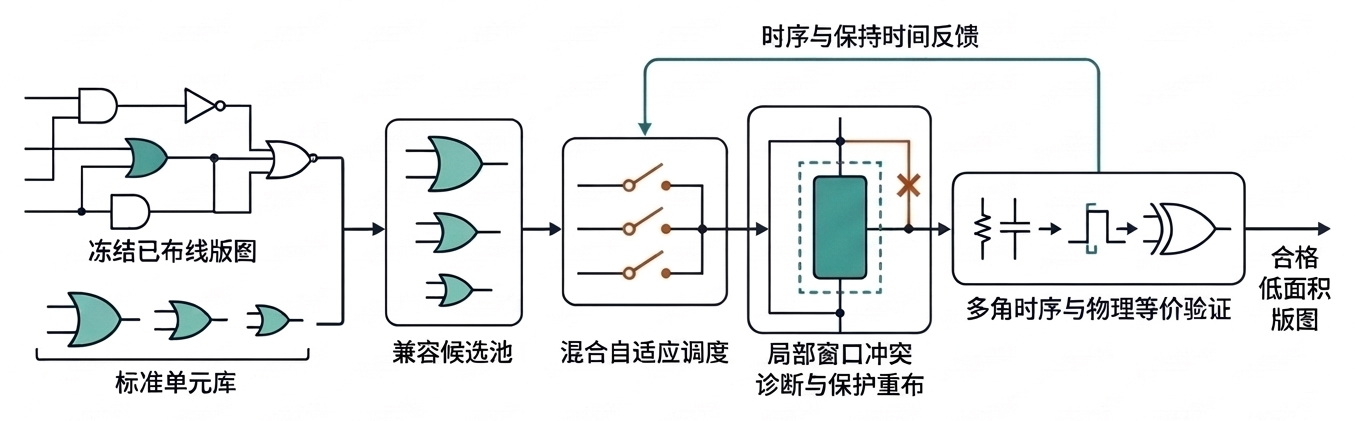
\includegraphics[width=0.92\textwidth]{tcad_20261126/fig1_framework_v4.png}
\caption{FAECO闭环系统架构示意图。框架以冻结已布线版图与标准单元库为起点构造互异实例兼容候选池，经混合自适应调度（有界乐观全池探针与保持时间反馈微批次）、行高自适应$1.0\times H_{\mathrm{row}}$局部窗口冲突诊断与保护式局部重布线、以及多角时序与物理等价验证，依据时序与保持时间反馈持续更新合格低面积版图检查点。}
\label{fig:arch}
\end{figure*}

\subsection{跨库兼容降尺寸枚举与初始前沿构建}

FAECO支持两类候选生成模式并共用同一在线物理验证闭环：
\begin{itemize}
\item \textbf{独立全库枚举模式：} 不依赖上游工具日志，直接解析冻结网表与标准单元库，过滤填充、阱接触、时钟树及虚拟负载单元，依据逻辑功能等价性、端口映射、同站点行高与严格更小物理宽度枚举低驱动替换，并对每个实例仅保留唯一最高优先级目标（确保$K$项池中实例两两互异）。随后在冻结寄生上执行单门快速预筛，滤除静态违反建立时间或电气约束的候选形成候选池$\mathcal{P}$。主实验统一取$K=18$（按默认批宽$b=3$对应6个完整微批次），第~\ref{sec:tc_sens}节进一步考察$K\in\{9,18,36\}$的扩展行为。全部预筛时间均足额计入各策略的720\,s墙钟预算。
\item \textbf{选择性回退模式：} 存在上游时序修复记录时，以被放大单元原尺寸为回退候选，在冻结寄生上以安全系数$\alpha=1.5$累积筛选，并采用$O(\log m)$前缀二分隔离多门耦合“转折门”后继续续跑后缀，将排查复杂度由$O(m)$降至$O(M(1+\log m))$。
\end{itemize}

进入物理验证前，框架支持两类初始排序接口：沿用冻结预筛的面积收益降序，或基于冻结典型角输出引脚建立时间裕量执行轻量灵敏度起序（排序开销全额计入对应策略预算）。设$m_i$为实例$i$各输出引脚最差建立时间松弛减去参考WNS（单位ps），灵敏度评分定义为
\begin{equation}
\label{eq:sens_rank}
\mathrm{score}_{\mathrm{init}}(i) = \Delta A_i \cdot \left(0.1 + \frac{\max(m_i,\,0)}{200\text{\,ps}}\right).
\end{equation}
其中，无量纲底数$0.1$保证零裕量非负候选仍保留非零基础权重，特征归一化尺度$200$\,ps与主流开源基准路径松弛分布量级匹配（去截顶设计避免高裕量候选在$200$\,ps处饱和同分），优先将$m_i>5$\,ps的非关键高收益单元置于前沿。

\subsection{行高自适应\texorpdfstring{$1.0\times H_{\mathrm{row}}$}{1.0 H\_row}局部窗口化DRC诊断与理论分析}
\label{sec:boxed_drc}

跨占位降尺寸引发的布线前局部冲突源于新单元引脚/障碍几何与周边已布线金属线的空间干涉（图~\ref{fig:drc_mech}）。设累计替换提议为$S$，被编辑实例集为$\mathcal{I}(S)$，与$\mathcal{I}(S)$引脚直连的非时钟信号网集为$\mathcal{D}(S)$。在冻结版图副本上对$\mathcal{I}(S)$执行原地单元替换并仅擦除$\mathcal{D}(S)$的旧走线，得到布线前预览几何集$G_{\mathrm{preview}}(S)$。为消除全块布线前DRC扫描随芯片面积线性膨胀的固定开销，本文导出行高自适应局部窗口诊断机制，其理论适用范围由命题~1严格刻画：

\begin{figure*}[t]
\centering
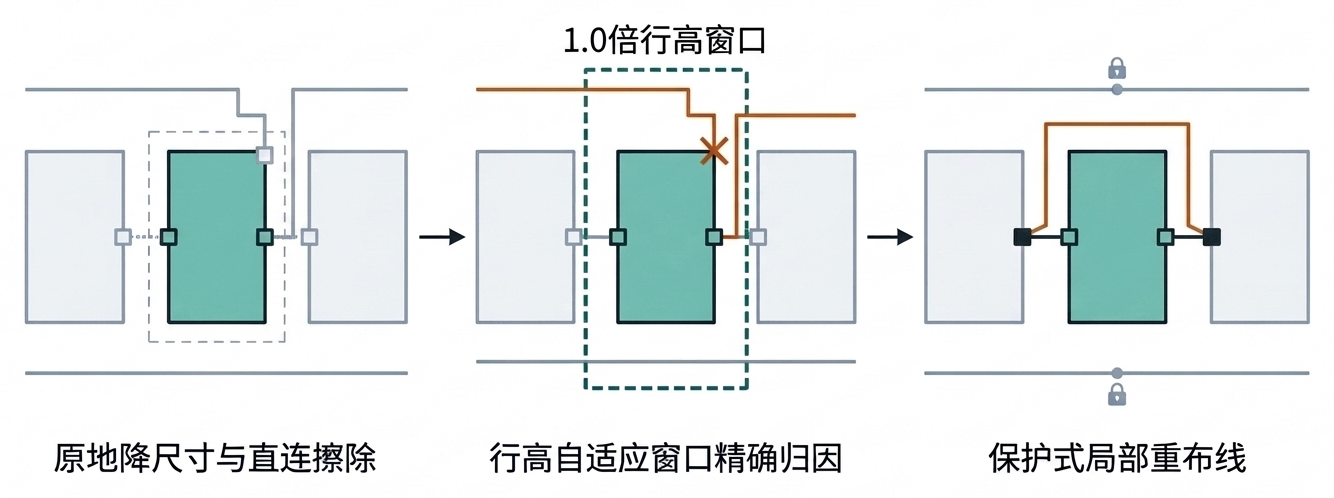
\includegraphics[width=0.90\textwidth]{tcad_20261126/fig2_boxed_drc_mechanism_v4.png}
\caption{行高自适应$1.0\times H_{\mathrm{row}}$局部窗口化冲突诊断与保护式局部重布线机理示意图。左：目标单元原地等效降尺寸（邻居零位移）并擦除直连旧线；中：以$1.0\times H_{\mathrm{row}}$局部窗口精确归因穿越或紧邻新引脚的真冲突邻网；右：仅放行直连网与DRC标记归因冲突邻网执行局部重布线，其余无冲突邻网严格维持几何锁定态。}
\label{fig:drc_mech}
\end{figure*}

\medskip
\noindent\textbf{命题 1（局部窗口对引脚层短路与成对间距规则的覆盖完备性）。} 记冻结参考版图与布线前预览版图的金属/过孔几何集合分别为$G_R$与$G_{\mathrm{preview}}(S)$，定义几何变化支撑集为对称差$\Delta G(S) = G_{\mathrm{preview}}(S)\triangle G_R$，并设标准单元替换所涉及的引脚与底层障碍层集合为$\mathcal{L}_{\mathrm{pin}}$。假定满足三项前提：（i）\textbf{起点清零}——参考$R$全块DRC违例数为零；（ii）\textbf{原地零位移}——预览仅对$g\in\mathcal{I}(S)$执行原地单元替换，所有非目标实例$g'\notin\mathcal{I}(S)$的坐标保持不变；（iii）\textbf{局部成对规则单调性}——仅针对有限作用半径$r_{\mathrm{drc}}(\ell)$的局部金属短路（$r=0$）与成对最小间距/平行长间距/端头间距/过孔间距规则（删除$\mathcal{D}(S)$的旧导体几何不会在远离$\mathcal{I}(S)$的未改动导体对之间制造新的短路或成对间距违例）。若标准单元行高$H_{\mathrm{row}}$满足
\begin{equation}
\label{eq:hrow_cond}
\max_{\ell\in\mathcal{L}_{\mathrm{pin}}} r_{\mathrm{drc}}(\ell) \le H_{\mathrm{row}},
\end{equation}
则替换$S$在布线前于$\mathcal{L}_{\mathrm{pin}}$上新增的全部短路与成对间距违例均完全包含于局部合并窗口集合$\mathcal{M}(S)$内。

\noindent\textbf{证明。} 设$v$为预览版图$G_{\mathrm{preview}}(S)$中在层$\ell\in\mathcal{L}_{\mathrm{pin}}$上出现的一处局部短路或成对间距违例，关联两导体图形$p_1,p_2\subseteq G_{\mathrm{preview}}(S)$，其欧氏距离$d(p_1,p_2)<r_{\mathrm{drc}}(\ell)$。若$p_1,p_2\subseteq G_R$均未发生改变，则由前提（iii）的局部成对规则性质，该违例必然已存在于$G_R$中，与前提（i）$R$全块DRC为零矛盾。故$p_1,p_2$中至少有一者属于新增几何$G_{\mathrm{preview}}(S)\setminus G_R \subseteq \Delta G(S)$。由前提（ii）与预览仅擦除$\mathcal{D}(S)$且仅原地替换$g\in\mathcal{I}(S)$，任何新增金属/引脚几何均严格位于被替换实例的物理边界框$\bigcup_{g\in\mathcal{I}(S)}\mathrm{BBox}(g)$内。从而违例$v$的局部空间支撑集（含关联双方交互邻域）必包含于以$r_{\mathrm{drc}}(\ell)$为半径的闵可夫斯基膨胀区域：
\begin{equation}
\label{eq:minkowski}
\mathrm{supp}(v) \subseteq \Bigl(\bigcup_{g\in\mathcal{I}(S)}\mathrm{BBox}(g)\Bigr)\oplus B\bigl(r_{\mathrm{drc}}(\ell)\bigr).
\end{equation}
令每个被替换实例$g\in\mathcal{I}(S)$的包围盒$[x_l,y_b,x_r,y_t]$向四向各外扩$\delta = 1.0\times H_{\mathrm{row}}$并裁剪至芯片有效区域$\mathrm{DieArea}$：
\begin{equation}
\label{eq:box}
\mathcal{B}(g) = \bigl[x_l-\delta,\; y_b-\delta,\; x_r+\delta,\; y_t+\delta\bigr]\cap \mathrm{DieArea},
\end{equation}
并对$\{\mathcal{B}(g)\mid g\in\mathcal{I}(S)\}$迭代合并重叠或接触矩形得到不相交窗口集合$\mathcal{M}(S)$。结合条件~\eqref{eq:hrow_cond}，有$B\bigl(r_{\mathrm{drc}}(\ell)\bigr)\subseteq [-\delta,\delta]^2$，故式~\eqref{eq:minkowski}右侧严格包含于$\bigcup_{g\in\mathcal{I}(S)}\mathcal{B}(g) \subseteq \bigcup_{B_j\in\mathcal{M}(S)}B_j$，证毕。$\blacksquare$

\medskip
需要强调两项严谨边界：首先，命题~1仅覆盖局部短路与成对间距类规则，不将擦除单调性无条件推广至最小面积（min-area）、最小步长（min-step）或全局金属密度规则；其次，式~\eqref{eq:hrow_cond}须按实际工艺技术LEF规则逐层核验，而非假设行高天然覆盖任意工艺的全部高层规则。表~\ref{tab:lef_rules}给出了对本文两种实验工艺真实技术LEF文件的逐层规则核验结果：在130\,nm SKY130HD（$H_{\mathrm{row}}=2.72\,\mu\text{m}$）上，从底层引脚层\texttt{li1}/\texttt{mcon}/\texttt{met1}（$\le 0.28\,\mu\text{m}$，9.7倍安全余量）直至最高层\texttt{met5}（$1.60\,\mu\text{m}$）全栈均满足式~\eqref{eq:hrow_cond}；在7\,nm ASAP7（$H_{\mathrm{row}}=0.27\,\mu\text{m}$）上，全部标准单元引脚层与中下层信号层\texttt{V0}--\texttt{V7}、\texttt{M1}--\texttt{M7}（引脚层\texttt{M1}--\texttt{M3}仅$0.018\,\mu\text{m}$，达15倍安全余量；\texttt{M4}--\texttt{M7}含EOL与平行长间距上限$0.072\,\mu\text{m}$）均严格满足式~\eqref{eq:hrow_cond}，仅不参与标准单元引脚修改的高层全局/电源层\texttt{M8}/\texttt{M9}（$1.0\,\mu\text{m}$）与\texttt{Pad}（$3.0\,\mu\text{m}$）超出$H_{\mathrm{row}}$。此外，局部窗口化仅用于布线前冲突预诊，候选重布线完成后终检一律恢复完整布线态并执行\textbf{全芯片独立全块DRC}，从而对所有制造规则（含最小面积与重布线次生违例）提供完整保障。

\begin{table}[t]
\centering
\caption{SKY130HD与ASAP7真实技术LEF逐层成对DRC作用半径与$1.0\times H_{\mathrm{row}}$覆盖核验}
\label{tab:lef_rules}
\scriptsize\setlength{\tabcolsep}{2.5pt}
\resizebox{\columnwidth}{!}{%
\begin{tabular}{llrrrrrc}
\toprule
\textbf{工艺与$H_{\mathrm{row}}$} & \textbf{代表层（类型）} & \textbf{最小间距} & \textbf{PRL上限} & \textbf{EOL间距} & \textbf{过孔间距} & \textbf{最大半径} & \textbf{$\le H_{\mathrm{row}}$} \\
 & & \textbf{/\textmu m} & \textbf{/\textmu m} & \textbf{/\textmu m} & \textbf{/\textmu m} & \textbf{/\textmu m} & \\
\midrule
\multirow{4}{*}{\shortstack[l]{SKY130HD\\($2.72\,\mu\text{m}$)}}
 & \texttt{li1}/\texttt{met1}（引脚层） & --- & 0.17 / 0.28 & --- & --- & 0.28 & 是（$9.7\times$） \\
 & \texttt{mcon}/\texttt{via}（过孔） & --- & --- & --- & 0.19 / 0.17 & 0.19 & 是 \\
 & \texttt{met2}--\texttt{met4}（信号） & --- & 0.28--0.40 & --- & --- & 0.40 & 是 \\
 & \texttt{via4}/\texttt{met5}（顶层） & --- & 1.60 & --- & 0.80 & 1.60 & 是 \\
\midrule
\multirow{4}{*}{\shortstack[l]{ASAP7\\($0.27\,\mu\text{m}$)}}
 & \texttt{M1}--\texttt{M3}（引脚/低层） & 0.018 & --- & --- & --- & 0.018 & 是（$15\times$） \\
 & \texttt{V0}--\texttt{V2}/\texttt{V7}（过孔） & --- & --- & --- & 0.018 / 0.046 & 0.046 & 是 \\
 & \texttt{M4}--\texttt{M7}（中层信号） & 0.024--0.032 & 0.072 & 0.024 & --- & 0.072 & 是（$3.8\times$） \\
 & \texttt{M8}/\texttt{M9}/\texttt{Pad}（高层） & --- & 1.00 / 3.00 & --- & --- & 3.00 & 否（非引脚层） \\
\bottomrule
\end{tabular}%
}
\end{table}

在邻网归因环节，对合并窗口集合$\mathcal{M}(S)$逐窗调用局部DRC并按规范键（违例类型、包围盒、关联对象）去重汇总。仅当全部检出标记均明确归属至$\mathcal{I}(S)$或其直连线网且关联至少一条已布线非时钟邻网时，提取这些邻网的并集作为\textbf{基于DRC标记归因的冲突邻网集合}$\mathcal{E}(S)$（注：并集提取给出由DRC标记直接指认的冲突邻网集，不声称在一般多解情形下构成理论最小基数子集），构造首次局部重布线的精确放行集合$\mathcal{R}_0(S)=\mathcal{D}(S)\cup\mathcal{E}(S)$，其余全部信号与时钟网严格维持几何锁定态。

\subsection{保护式局部重布线与混合自适应微批次调度}
\label{sec:sched}

在保护式局部重布线后端中，每次验证均从同一冻结参考$R$出发，应用累计替换集$S$并仅放行$\mathcal{R}_0(S)$，依次执行局部引脚接入、局部详细重布线、全芯片寄生重提取与三工艺角STA。若首轮重布后独立全块DRC仍检出由新走线引发的次生违例，后端依据新增标记增补对应非时钟邻网并至多执行一次定向复修；全部门控通过后再执行全网表两态SEC。

为兼顾全池一次可交付场景的吞吐上限与高脆弱设计上的跨角稳健性，本文设计了\textbf{混合自适应调度框架（Hybrid FAECO，算法~\ref{alg:faeco}）}，由两阶段耦合构成：
\begin{enumerate}
\item \textbf{阶段一：有界乐观全池探针（Bounded Optimistic Probe）。} 进入搜索预算后，首先在$1.0\times H_{\mathrm{row}}$窗口保护后端上以单遍无复修模式尝试提交完整候选池$\mathcal{P}$，并施加严格探针子预算上限
\begin{equation}
\label{eq:probe_budget}
\tau_{\mathrm{probe}} = \min\bigl(180\text{\,s},\; 0.30\,(\tau_{\max} - t_{\mathrm{screen}})\bigr).
\end{equation}
若该单遍探针在$\tau_{\mathrm{probe}}$内通过全部多角时序、独立全块DRC、天线与SEC验证，则直接交付100\%候选池收益并提前结束；若出现任何时序/物理拒收或触及$\tau_{\mathrm{probe}}$，则立即终止并丢弃探针，将剩余全部墙钟预算无损移交阶段二。当用户优先追求极早时刻的随时可交付收益（Anytime AUC）时，亦可关闭阶段一退化为纯微批次模式（Pure FAECO）。
\item \textbf{阶段二：保持时间反馈自适应微批次与确定性去重。} 以微批次（默认批宽$b=3$）推进前沿：（a）\textbf{Hold失效暂缓与直连电容代理重排}——当多门批次因任一工艺角相对Hold WNS退化被拒时，将其压入暂缓队列$\mathcal{Q}_{\mathrm{def}}$以优先探索未访问前沿，并在首次触发相对Hold暂缓时按直连信号网总电容代理指标对未访问前沿执行一次稳定降序重排：
\begin{equation}
\label{eq:cap_rerank}
\mathrm{prio}(i) = \frac{\Delta A_i}{1 + C_i / \widetilde{C}},
\end{equation}
其中$C_i$为实例$i$直连非电源信号网在冻结寄生中的总电容之和，$\widetilde{C}$为候选池中位数。式~\eqref{eq:cap_rerank}作为低开销启发式代理特征（仅解析冻结寄生，耗时低于0.1\,s），在保持高面积收益的同时倾向于规避高扇出/高寄生负载网扰动，其独立收益由第~\ref{sec:geo_ablation}节受控消融验证；（b）\textbf{Setup失效原位二分与确定性拒收去重}——若多门批次仅因建立时间超预算被拒，算法将其原位二分为左右子批压入前沿栈头，同时以规范化排序动作元组为键将该累计动作集记入确定性拒收集合$\mathcal{K}_{\mathrm{setup}}$。由于所有验证均从同一冻结参考、固定4线程布线及确定性规则启动，后续拆分重构出$\mathcal{K}_{\mathrm{setup}}$中同一规范化动作集时直接跳过物理调用并继续二分。
\end{enumerate}

\paragraph{严格墙钟截止与子进程预算裁剪}
为确保实际运行严格遵守$\tau_{\max}=720$\,s上限而非事后截取统计，调度器在每次派发下游子进程（窗口DRC预检、局部重布/RCX、三工艺角STA、独立全块DRC与SEC）前，均实时计算剩余墙钟$t_{\mathrm{rem}} = \tau_{\max} - t_{\mathrm{now}}$，并将有效操作系统超时参数裁剪为$\min(\tau_{\mathrm{stage}},\, t_{\mathrm{rem}})$直接传递给子进程。一旦子进程因墙钟裁剪超时或返回时刻达到$\tau_{\max}$，控制层立即强制终止未完成子进程、丢弃未完结候选并结束搜索，确保检查点落盘与总墙钟统计严格位于$\tau_{\max}$以内。

\begin{algorithm}[t]
\caption{Hybrid FAECO：有界乐观探针与局部窗口自适应微批次}
\label{alg:faeco}
\scriptsize\linespread{1.03}\selectfont
\begin{algorithmic}[1]
\Require 冻结参考 $R$，互异池 $\mathcal{P}$，批宽 $b=3$，时限 $\tau_{\max}$，预算 $(B_W,B_{T,v})$，探针开关 $\mathrm{probe}$
\Ensure 随时可交付的最佳ECO合格端点 $(S^*, F^*)$
\State 初始化前沿排序（面积序或式~\eqref{eq:sens_rank}灵敏度序）；$S^* \gets \emptyset$，$F^* \gets R$
\If{$\mathrm{probe}$} \Comment{阶段一：有界乐观全池探针}
    \State 设 $\tau_{\mathrm{probe}} \gets \min(180\text{\,s},\, 0.30(\tau_{\max}-t_{\mathrm{screen}}))$；在$1.0H_{\mathrm{row}}$窗口后端单遍验证 $\mathcal{P}$
    \If{在 $\tau_{\mathrm{probe}}$ 内满足式~\eqref{eq:obj}全部约束} \Return $(\mathcal{P}, F(\mathcal{P}))$ \EndIf
\EndIf
\State $\mathcal{Q}_{\mathrm{def}} \gets []$，$\mathcal{K}_{\mathrm{setup}} \gets \emptyset$，$\mathrm{reranked} \gets \mathrm{false}$，构建批宽 $b$ 微批次队列 $\mathcal{Q}$
\While{$t_{\mathrm{rem}} > 0$ 且（$\mathcal{Q}$ 非空或 $\mathcal{Q}_{\mathrm{def}}$ 非空）}
    \State 从 $\mathcal{Q}$ 弹出 $B$（$\mathcal{Q}$ 空则从 $\mathcal{Q}_{\mathrm{def}}$ 弹出并二分）；$S \gets \mathrm{sort}(S^* \cup B)$
    \If{$S \in \mathcal{K}_{\mathrm{setup}}$} \Comment{确定性Setup拒收去重}
        \State 若 $|B|>1$ 将 $B$ 二分压回 $\mathcal{Q}$ 头部；\textbf{continue}
    \EndIf
    \State 在 $R$ 副本上原地替换 $\mathcal{I}(S)$、擦除 $\mathcal{D}(S)$，由式~\eqref{eq:box}生成 $\mathcal{M}(S)$ 并归因冲突邻网 $\mathcal{E}(S)$
    \State 锁定外围线网，仅重布 $\mathcal{D}(S)\cup\mathcal{E}(S)$（至多复修1次），执行RCX、三工艺角STA、独立全块DRC、天线与SEC（子进程限时裁剪至 $t_{\mathrm{rem}}$）
    \If{未超时且满足式~\eqref{eq:obj}全部约束}
        \State $S^* \gets S$，$F^* \gets F(S)$ \Comment{更新ECO合格检查点}
    \ElsIf{$|B|>1$ 且拒因含任一角相对Hold WNS退化}
        \State 将 $B$ 追加至 $\mathcal{Q}_{\mathrm{def}}$；若 $\neg\mathrm{reranked}$ 则按式~\eqref{eq:cap_rerank}重排未访问前沿并置 $\mathrm{reranked}\gets\mathrm{true}$
    \Else
        \State 若仅因建立时间超预算拒收则 $\mathcal{K}_{\mathrm{setup}} \gets \mathcal{K}_{\mathrm{setup}} \cup \{S\}$
        \State 若 $|B|>1$ 则将二分结果 $B_L, B_R$ 按序压入 $\mathcal{Q}$ 头部
    \EndIf
\EndWhile
\State \Return $(S^*, F^*)$
\end{algorithmic}
\end{algorithm}

% ============================================================
% §5 实验评估
% ============================================================
\section{实验评估}

\subsection{实验平台、复现配置与基准特征}

全部双工艺布线后实验在统一Linux工作站上运行（AMD Ryzen~7 7435H处理器，WSL2内存11\,GiB；实验进程独占6个物理核心、固定详细布线为4线程，全部子进程按系统单调时钟串行计时以消除并发负载干扰）。底层开源工具链与工艺平台全局锁定：OpenROAD（提交\texttt{b511b6a2}，内嵌TritonRoute-WXL\cite{tritonroutewxl}与OpenRCX，详细布线迭代上限64轮）、OpenSTA~3.1.0\cite{sta}、Yosys~0.70+255（全网表两态SEC\cite{yosys}）与OpenROAD-flow-scripts（提交\texttt{da8f092a}）。SKY130HD采用\texttt{sky130\_fd\_sc\_hd}三工艺角时序库（FF $-40^\circ\text{C}/1.95\text{\,V}$、TT $25^\circ\text{C}/1.80\text{\,V}$、SS $-40^\circ\text{C}/1.40\text{\,V}$）与对应名义RCX规则文件；ASAP7采用7.5轨RVT多文件NLDM三工艺角时序库（FF/TT/SS）与ASAP7名义RCX规则文件。三工艺角STA共享同一详细布线后提取的名义SPEF文件。

主评估覆盖130\,nm SKY130HD与7\,nm ASAP7双工艺四个通过独立全块DRC=0、零天线与原生SEC验证的冻结基准（表~\ref{tab:benchmarks}），以及第~\ref{sec:tc_sens}节新增的\textbf{绝对时序收敛（Timing-closed）}7\,nm UART基准（500\,ps周期，三工艺角Setup/Hold均严格非负）。四个主基准均带有不同程度的初始典型角建立时间负松弛（表~\ref{tab:benchmarks}注），故主实验统一按第3.1节定义的\textbf{ECO合格状态}评测，而绝对收敛基准进一步检验\textbf{Timing-closed}状态保持能力。除特别标注外，主对照采用正反序配对执行，各策略均足额扣除同一公共预筛耗时并如实计入排序、诊断、重布、提取、STA、终检及SEC开销。

\begin{table*}[t]
\centering
\caption{双工艺布线后冻结基准设计特征、时序状态与预算配置（18项互异实例候选池）}
\label{tab:benchmarks}
\scriptsize\setlength{\tabcolsep}{3.0pt}
\resizebox{\textwidth}{!}{%
\begin{tabular}{llrrrrrrr}
\toprule
\textbf{基准模块（角色与状态）} & \textbf{工艺与$H_{\mathrm{row}}$} & \textbf{基线功能面积} & \textbf{信号线网 /} & \textbf{时钟周期} & \textbf{1\% Setup} & \textbf{基线Hold WNS} & \textbf{候选池上界} & \textbf{公共预筛} \\
 & & \textbf{/\textmu m$^2$} & \textbf{SEC等价点} & \textbf{/ps} & \textbf{预算/ps} & \textbf{(FF/TT/SS, ps)} & \textbf{/\textmu m$^2$} & \textbf{耗时/s} \\
\midrule
SKY130HD AES（高冲突，ECO参考） & 130\,nm / 2.72\,\textmu m & 116,507.99 & 15,657 / 11,089 & 3,600 & 36.0 & $+$336.3 / $+$523.9 / $+$55.3 & 197.6896 & 113.36 \\
SKY130HD \texttt{riscv32i}（处理器，ECO参考） & 130\,nm / 2.72\,\textmu m & 71,427.25 & 5,588 / 4,559 & 6,000 & 60.0 & $+$373.4 / $+$579.2 / $+$2019.3 & 147.6416 & 64.10 \\
ASAP7 UART（7\,nm外设，ECO参考） & 7\,nm / 0.27\,\textmu m & 79.01 & 797 / 567 & 270 & 2.7 & $+$50.3 / $+$67.5 / $+$54.1 & 1.18098 & 81.56 \\
ASAP7 AES（7\,nm留出，ECO参考） & 7\,nm / 0.27\,\textmu m & 1,181.81 & 12,412 / 10,027 & 380 & 3.8 & $+$35.4 / $+$52.1 / $+$24.7 & 1.76418 & 156.27 \\
ASAP7 UART-TC（7\,nm，\textbf{Timing-closed}） & 7\,nm / 0.27\,\textmu m & 79.01 & 797 / 567 & 500 & 5.0 & $+$50.3 / $+$67.5 / $+$54.1 & 1.18098 & 81.56 \\
\bottomrule
\end{tabular}%
}

\vspace{2pt}
\parbox{\textwidth}{\footnotesize 注：全部基准均满足独立全块DRC=0、天线=0与原生SEC全证，且18项候选池经核验全部由18个互异实例构成。前四基准冻结起点典型角Setup WNS依次为$-380.5$、$-474.2$、$-39.6$与$-153.1$\,ps（处于残留负松弛参考态）；ASAP7 UART-TC三工艺角Setup WNS依次为$+255.85$、$+190.42$与$+30.29$\,ps，三工艺角Setup/Hold均严格非负。}
\end{table*}

\subsection{跨工艺全景对照、离线LR解耦与Hybrid FAECO实证}
\label{sec:main_results}

本节在双工艺四个主基准上系统对比原生功耗回收、离线五轮冻结寄生拉格朗日松弛（LR）、灵敏度单门、固定微批次、纯微批次FAECO及Hybrid FAECO。其中，经典冻结寄生LR基线\cite{chen1999fast,flach2014effective}在冻结典型角SPEF上对同一18项池执行5轮次梯度迭代：初始拉格朗日乘子$\lambda_i^{(0)}=1.0$，每轮依引脚建立时间违例比$\nu_i = \bigl(W_{\mathrm{tgt}}-s_i\bigr)/\max(10,|W_{\mathrm{TT}}(R)|)$按$\lambda_i \leftarrow \mathrm{clip}\bigl(\lambda_i\exp(\mathrm{clip}(2\nu_i,-2,3)),\,0.05,\,1000\bigr)$更新，并以拉格朗日净收益$\Delta A_i - 0.01\lambda_i\max(0, W_{\mathrm{TT}}(R)-W_{\mathrm{TT}}^{\mathrm{new}})>0$且满足冻结Setup/Hold门控决定单元替换提交。需要透明指出，由于18项池已预先通过单门冻结预筛，五轮离线LR在全部四个基准上均选择了18/18项候选（耗时1.5--5.0\,s），从而在冻结预筛池上与“全池18门直接提交”等价。

图~\ref{fig:anytime}、表~\ref{tab:main_overview}与表~\ref{tab:lr_hybrid}汇总了720\,s限时全景结果与后端/前端解耦对照，揭示出四项核心发现：

\begin{figure*}[t]
\centering
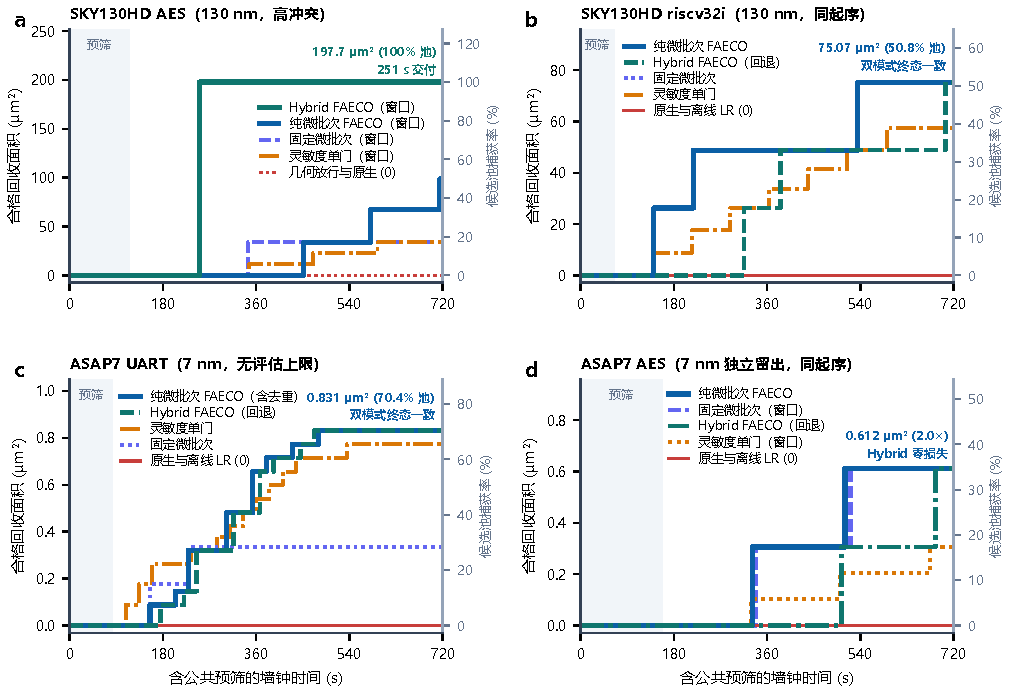
\includegraphics[width=0.94\textwidth]{tcad_20261126/fig3_anytime_curves_v4_zh.pdf}
\caption{双工艺四个主基准在720\,s墙钟预算内的随时可交付ECO合格回收曲线（正序实测，阴影区为公共预筛开销，右轴为18项候选池捕获率）。（a）SKY130HD AES上同一$1.0\times H_{\mathrm{row}}$窗口后端对比，Hybrid FAECO在251\,s交付100\%池收益（197.7\,\textmu m$^2$）；（b）SKY130HD \texttt{riscv32i}；（c）ASAP7 UART；（d）7\,nm独立留出ASAP7 AES，展示同一窗口后端下固定微批次、纯微批次FAECO与Hybrid FAECO的回退零损失特性。}
\label{fig:anytime}
\end{figure*}

\begin{table*}[t]
\centering
\caption{双工艺四主基准720\,s全景对照：ECO合格面积、功能单元/候选池降幅、时间平均收益、预算利用率与提取寄生功耗}
\label{tab:main_overview}
\scriptsize\setlength{\tabcolsep}{2.8pt}
\resizebox{\textwidth}{!}{%
\begin{tabular}{llrrrrrl}
\toprule
\textbf{基准模块} & \textbf{方法与后端配置} & \textbf{合格面积} & \textbf{功能面积 / 池} & \textbf{时间平均} & \textbf{Setup预算} & \textbf{TT提取功耗变化（已交付端点）} & \textbf{独立DRC/天线} \\
 & & \textbf{/\textmu m$^2$（门数）} & \textbf{（\% / \%）} & \textbf{收益/\textmu m$^2$} & \textbf{利用率\%} & \textbf{（总/组合/漏电）或拒收诊断} & \textbf{/ SEC} \\
\midrule
\multirow{8}{*}{SKY130HD AES}
 & OpenROAD原生功耗回收（全片重布） & 0.0000（0） & 0.000 / 0.0 & 0.00 & 2,116\%（拒） & 拒收：SS Setup $-$761.8\,ps、三角Hold退化 & 0/0 / --- \\
 & 静态几何放行（$G_{k1}$ / $G_{r0}$） & 0.0000（0） & 0.000 / 0.0 & 0.00 & Hold拒 & 拒收：过度放行致SS Hold $-$10.48\,ps & 0/0 / --- \\
 & 灵敏度单门（$1.0H_{\mathrm{row}}$窗口） & 33.7824（3） & 0.029 / 17.1 & 11.72 & 0.00\% & ---（已交付3门） & 0/0 / 11,089 \\
 & 固定微批次（$1.0H_{\mathrm{row}}$窗口） & 33.7824（3） & 0.029 / 17.1 & 17.62 & 0.00\% & ---（已交付3门） & 0/0 / 11,089 \\
 & 全块诊断FAECO & 67.5648（6） & 0.058 / 34.2 & 16.24 & 0.24\% & $-$0.036\% / $-$0.049\% / $-$0.022\% & 0/0 / 11,089 \\
 & 纯微批次FAECO（$1.0H_{\mathrm{row}}$窗口） & 98.8448（9） & 0.085 / 50.0 & 19.37 & 0.23\% & $-$0.051\% / $-$0.071\% / $-$0.032\% & 0/0 / 11,089 \\
 & \textbf{Hybrid FAECO（$1.0H_{\mathrm{row}}$窗口）} & \textbf{197.6896（18）} & \textbf{0.170 / 100.0} & \textbf{128.78} & \textbf{0.10\%} & \textbf{全池18门（251\,s交付）} & \textbf{0/0 / 11,089} \\
\midrule
\multirow{5}{*}{SKY130HD \texttt{riscv32i}}
 & OpenROAD原生功耗回收（全片重布） & 0.0000（0） & 0.000 / 0.0 & 0.00 & TNS超9.4$\times$ & 拒收：TT TNS超预算且新增1处天线 & 0/1 / --- \\
 & 灵敏度单门（同起序） & 57.5552（7） & 0.081 / 39.0 & 28.80 & 0.22\% & ---（已交付7门） & 0/0 / 4,559 \\
 & 固定微批次（同起序） & 75.0720（9） & 0.105 / 50.8 & 43.61 & 0.73\% & $-$0.042\% / $-$0.205\% / $-$0.092\% & 0/0 / 4,559 \\
 & \textbf{纯微批次FAECO（同起序）} & \textbf{75.0720（9）} & \textbf{0.105 / 50.8} & \textbf{43.59} & \textbf{0.73\%} & \textbf{$-$0.042\% / $-$0.205\% / $-$0.092\%} & \textbf{0/0 / 4,559} \\
 & Hybrid FAECO（探针截断回退） & 75.0720（9） & 0.105 / 50.8 & 25.81 & 0.73\% & 同9门端点（探针180\,s截断回退） & 0/0 / 4,559 \\
\midrule
\multirow{5}{*}{ASAP7 UART}
 & OpenROAD原生功耗回收（全片重布） & 0.00000（0） & 0.000 / 0.0 & 0.000 & Hold拒 & 拒收：16处同面积替换致FF/TT Hold退化 & 0/0 / --- \\
 & 固定微批次（无评估上限） & 0.33534（6） & 0.424 / 28.4 & 0.246 & 49.9\% & ---（已交付6门） & 0/0 / 567 \\
 & 灵敏度单门（无评估上限） & 0.77274（12） & 0.978 / 65.4 & 0.464 & 50.6\% & ---（已交付12门） & 0/0 / 567 \\
 & \textbf{纯微批次FAECO（含去重）} & \textbf{0.83106（13）} & \textbf{1.052 / 70.4} & \textbf{0.482} & \textbf{50.5\%} & \textbf{$-$0.660\% / $-$2.142\% / $-$0.777\%} & \textbf{0/0 / 567} \\
 & Hybrid FAECO（探针快速回退） & 0.83106（13） & 1.052 / 70.4 & 0.466 & 50.5\% & 同13门端点（探针26.1\,s拒收回退） & 0/0 / 567 \\
\midrule
\multirow{6}{*}{ASAP7 AES（留出）}
 & OpenROAD原生功耗回收（全片重布） & 0.00000（0） & 0.000 / 0.0 & 0.000 & 重布超时 & 拒收：全片重布超时且连通性断路 & 失败 / --- \\
 & 全块灵敏度单门（同起序） & 0.20412（2） & 0.017 / 11.6 & 0.051 & 0.00\% & ---（已交付2门） & 0/0 / 10,027 \\
 & 灵敏度单门（$1.0H_{\mathrm{row}}$窗口） & 0.30618（3） & 0.026 / 17.4 & 0.093 & 5.75\% & ---（已交付3门） & 0/0 / 10,027 \\
 & 固定微批次（$1.0H_{\mathrm{row}}$窗口） & 0.61236（6） & 0.052 / 34.7 & 0.247 & 6.33\% & 同6门端点（微批次摊销贡献） & 0/0 / 10,027 \\
 & \textbf{纯微批次FAECO（$1.0H_{\mathrm{row}}$窗口）} & \textbf{0.61236（6）} & \textbf{0.052 / 34.7} & \textbf{0.254} & \textbf{6.33\%} & \textbf{$-$0.017\% / $-$0.023\% / $-$0.014\%} & \textbf{0/0 / 10,027} \\
 & Hybrid FAECO（探针截断回退） & 0.61236（6） & 0.052 / 34.7 & 0.107 & 6.33\% & 同6门端点（探针169\,s截断回退） & 0/0 / 10,027 \\
\bottomrule
\end{tabular}%
}

\vspace{2pt}
\parbox{\textwidth}{\footnotesize 注：同一基准各行共享完全一致的冻结参考、18项互异候选池、720\,s墙钟与全项验证门控；\texttt{riscv32i}与ASAP7 AES统一采用式~\eqref{eq:sens_rank}现场同灵敏度起序。功耗针对各基准已交付代表性最优端点于TT提取寄生下测算，失败方法列示具体拒收原因。}
\end{table*}

\begin{enumerate}
\item \textbf{离线LR后端解耦与Hybrid FAECO的跨设计支配优势。} 表~\ref{tab:lr_hybrid}清晰揭示了物理后端与搜索前端的协同规律：在SKY130HD AES上，脱离保护后端的独立LR（标准全片重布）在600\,s内超时失效；而挂载FAECO的$1.0\times H_{\mathrm{row}}$窗口保护后端后，18门全池提交仅需8.22\,s窗口预检即归因7条冲突邻网，并在140.90\,s内一次通过全部验证（197.6896\,\textmu m$^2$，SS Hold反向改善$+0.459$\,ps）。该现象表明保持时间可行域对子集拓扑具有非单调性——全池18门联合重布改变了局部互连拓扑从而跨过了小批次的保持时间敏感区。然而，在其余3/4设计上，即使配备同一窗口保护后端，一次性全池/LR提交仍全部失效（\texttt{riscv32i}重布超时、UART快角Setup越界且典型/慢角Hold退化、ASAP7 AES耗时463.85\,s仍因慢角Hold拒收）。引入有界乐观探针后，\textbf{Hybrid FAECO在SKY130HD AES上251\,s内直达100\%候选池（197.6896\,\textmu m$^2$，时间平均收益跃升6.65倍至128.78\,\textmu m$^2$），同时在其余3/4基准上于子预算内干净截断并无损回退，实现4/4设计终态合格面积严格持平或2.00倍超越纯微批次FAECO}。两者亦构成清晰帕累托权衡：Hybrid FAECO在终态回收上全面占优或持平，而纯微批次FAECO在探针注定失败的万门设计（\texttt{riscv32i}、ASAP7 AES）上具有更高的早窗时间平均收益（43.59对25.81、0.254对0.107\,\textmu m$^2$）。
\item \textbf{高候选池捕获率与极低时序裕量消耗。} 在720\,s内，Hybrid/纯微批次FAECO在四基准上捕获候选池上界的34.7\%--100.0\%，三个万门级基准上的实际最大跨角建立时间损失仅占用允许预算的0.10\%--6.33\%，全部交付端点的三工艺角Hold WNS均维持非负且无退化。
\item \textbf{面积与提取寄生功耗协同下降。} 全部四个基准的已交付端点在TT提取寄生下实现总功耗、组合逻辑功耗与静态漏电同步下降（如ASAP7 UART组合逻辑功耗降低2.142\%）。
\item \textbf{单角原生功耗回收在多角闭环下的系统性失效。} OpenROAD内置功耗回收引擎在全部四个基准上（无论是否放宽建立时间选项）均未能交付合格解；须客观说明，原生引擎执行全片重布而非本文保护式局部重布，其失效由单角冻结寄生误判与无保护全片扰动共同导致。早期开源尺寸器TritonSizer因依赖旧版闭源字节码组件与特定解析接口，未能直接接入当前多角详细重布线流程。
\end{enumerate}

\begin{table*}[t]
\centering
\caption{离线LR/全池直提、纯微批次FAECO与Hybrid FAECO在四设计上的解耦对照（720\,s，同一18项池）}
\label{tab:lr_hybrid}
\scriptsize\setlength{\tabcolsep}{3.4pt}
\resizebox{\textwidth}{!}{%
\begin{tabular}{llrrrl}
\toprule
\textbf{基准模块（工艺）} & \textbf{方法与后端配置} & \textbf{探针/离线耗时} & \textbf{720\,s合格面积} & \textbf{池捕获率} & \textbf{验证判定与失效/回退归因} \\
 & & \textbf{/s} & \textbf{/\textmu m$^2$（门数）} & \textbf{/\%} & \\
\midrule
\multirow{4}{*}{SKY130HD AES（130\,nm）}
 & 独立LR（标准全片重布） & $>$600.0 & 0.0000（0） & 0.0\% & 全芯片详细布线超时终止 \\
 & 离线LR/全池直提（挂载窗口后端） & 140.90 & 197.6896（18） & 100.0\% & 通过（窗口8.22\,s归因7邻网，SEC全证） \\
 & 纯微批次FAECO（窗口后端） & --- & 98.8448（9） & 50.0\% & 5轮微批次通过（AUC 19.37\,\textmu m$^2$） \\
 & \textbf{Hybrid FAECO（窗口后端）} & \textbf{137.60} & \textbf{197.6896（18）} & \textbf{100.0\%} & \textbf{阶段一探针通过直接早停（AUC 128.78\,\textmu m$^2$）} \\
\midrule
\multirow{3}{*}{SKY130HD \texttt{riscv32i}（130\,nm）}
 & 离线LR/全池直提（挂载窗口后端） & 245.62 & 0.0000（0） & 0.0\% & 18门一次修改诱发局部详细布线超时 \\
 & 纯微批次FAECO（窗口后端） & --- & 75.0720（9） & 50.8\% & 3批通过（AUC 43.59\,\textmu m$^2$） \\
 & \textbf{Hybrid FAECO（窗口后端）} & \textbf{180.15} & \textbf{75.0720（9）} & \textbf{50.8\%} & \textbf{子预算截断并回退，终态零损失（AUC 25.81）} \\
\midrule
\multirow{3}{*}{ASAP7 UART（7\,nm）}
 & 离线LR/全池直提（挂载窗口后端） & 25.58 & 0.00000（0） & 0.0\% & 快角Setup越界与典型/慢角Hold退化 \\
 & 纯微批次FAECO（窗口后端） & --- & 0.83106（13） & 70.4\% & 19轮自然收敛（AUC 0.482\,\textmu m$^2$） \\
 & \textbf{Hybrid FAECO（窗口后端）} & \textbf{26.11} & \textbf{0.83106（13）} & \textbf{70.4\%} & \textbf{快速拒收回退，终态零损失（AUC 0.466）} \\
\midrule
\multirow{3}{*}{ASAP7 AES（7\,nm留出）}
 & 离线LR/全池直提（挂载窗口后端） & 463.85 & 0.00000（0） & 0.0\% & 触发次生DRC复修且慢角Hold退化 \\
 & 纯微批次FAECO（窗口后端） & --- & 0.61236（6） & 34.7\% & 2批通过+第3批暴露Hold退化（AUC 0.254） \\
 & \textbf{Hybrid FAECO（窗口后端）} & \textbf{169.24} & \textbf{0.61236（6）} & \textbf{34.7\%} & \textbf{单遍无复修子预算截断回退，终态零损失（AUC 0.107）} \\
\bottomrule
\end{tabular}%
}
\end{table*}

\subsection{受控变量消融：邻网放行策略与同窗口调度组件分解}
\label{sec:geo_ablation}

为严格分离“局部窗口保护后端”与“自适应调度各组件”的独立贡献，我们在高冲突SKY130HD AES与7\,nm ASAP7 AES上开展了两组受控变量消融实验。

\paragraph{静态几何邻网放行与现场DRC归因对照}
首先在SKY130HD AES上对冻结版图全部非时钟信号网构建空间索引（耗时1.39\,s，单次查询低于1\,ms），以10组历史请求中在线DRC检出的26次真实冲突邻网为基准：最近邻规则$G_{k1}$仅召回46.2\%真冲突网却放行1.85倍邻网（48条）；底层接触规则$G_{r0}$达100\%召回但放行膨胀至3.19倍（83条）；双层接触规则$G_{\mathrm{low}}$放行高达15.77倍（410条）。在完全相同的FAECO调度、18项池与720\,s预算下开展六臂正反序完整物理对照，两类静态几何规则合格回收均为零，而现场DRC归因在正反两序均交付67.5648\,\textmu m$^2$。表~\ref{tab:geo_causal}与图~\ref{fig:ablation}(a)隔离了正序三臂在同一三门提议上的受控结果：$G_{k1}$因漏冲突触发复修（208.73\,s）且误放保护网致慢角Hold退化10.48\,ps；$G_{r0}$虽借0.02\,s预检实现零复修并将单轮耗时压至105.60\,s，但多余放行的6条无冲突保护网重布后同样令慢角Hold骤降10.48\,ps；唯有现场DRC归因精准锁定3条冲突邻网，一次通过并令三工艺角Hold WNS全部改善。进一步在“调度$\times$后端”$2\times 2$正反序交叉对照（表~\ref{tab:aes_factorial}）中，切入布线前DRC诊断使固定微批次与FAECO到达同一物理首达端点的墙钟分别提前72.4--84.0\,s和158.0--164.4\,s，首达前分别消除1次与2次冗余详细布线。这验证了本文的核心物理发现：\textbf{减少无冲突邻网重布可同时提升验证吞吐与多角保持时间稳定性}。

\begin{figure*}[t]
\centering
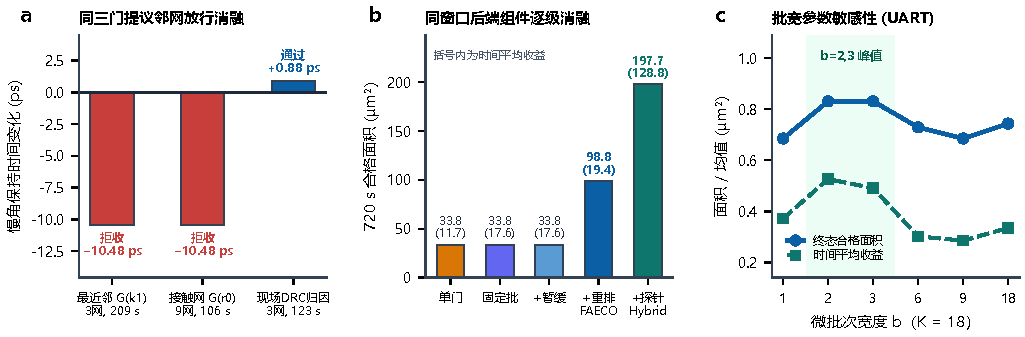
\includegraphics[width=0.94\textwidth]{tcad_20261126/fig4_ablation_v4_zh.pdf}
\caption{受控变量消融与参数敏感性实验结果。（a）SKY130HD AES同一三门提议上的邻网放行消融，表明过度放行无冲突邻网诱发$-10.48$\,ps慢角Hold退化；（b）SKY130HD AES同一$1.0\times H_{\mathrm{row}}$窗口后端下的五级调度组件消融（括号内为时间平均随时合格回收），量化微批次摊销、直连电容重排与有界乐观探针的独立增益；（c）ASAP7 UART上微批次宽度$b\in\{1,2,3,6,9,18\}$敏感性倒U曲线（$K=18$）。}
\label{fig:ablation}
\end{figure*}

\begin{table}[t]
\centering
\caption{SKY130HD AES同一三门候选提议上的邻网放行受控对比}
\label{tab:geo_causal}
\scriptsize\setlength{\tabcolsep}{2.3pt}
\resizebox{\columnwidth}{!}{%
\begin{tabular}{lrrrrc}
\toprule
\textbf{邻网放行} & \textbf{预放邻网} & \textbf{预检} & \textbf{本轮耗时} & \textbf{FF/TT/SS Hold WNS} & \textbf{验证} \\
\textbf{策略} & \textbf{（复修）} & \textbf{/s} & \textbf{/s} & \textbf{变化（ps）} & \textbf{判定} \\
\midrule
最近邻 $G_{k1}$ & 3（1次） & 0.02 & 208.73 & $-$0.41 / $-$0.64 / \textbf{$-$10.48} & 拒收 \\
接触邻网 $G_{r0}$ & 9（0次） & 0.02 & 105.60 & $-$0.40 / $-$0.62 / \textbf{$-$10.48} & 拒收 \\
\textbf{现场DRC归因} & \textbf{3（0次）} & 14.21 & 122.75 & \textbf{$+$0.05 / $+$0.08 / $+$0.88} & \textbf{通过} \\
\bottomrule
\end{tabular}%
}
\end{table}

\begin{table}[t]
\centering
\caption{SKY130HD AES调度$\times$后端$2\times 2$正反序交叉对照（720\,s）}
\label{tab:aes_factorial}
\scriptsize\setlength{\tabcolsep}{2.5pt}
\resizebox{\columnwidth}{!}{%
\begin{tabular}{llrrrrr}
\toprule
\textbf{调度策略} & \textbf{后端模式} & \textbf{窗内回收} & \multicolumn{2}{c}{\textbf{首达0.01\%/s}} & \multicolumn{2}{c}{\textbf{完成验证}} \\
\cmidrule(lr){4-5}\cmidrule(lr){6-7}
 & & \textbf{/\textmu m$^2$} & \textbf{正序} & \textbf{反序} & \textbf{正序} & \textbf{反序} \\
\midrule
固定微批次 & 常规复修 & 33.7824 & 448.64 & 443.27 & 3 & 3 \\
固定微批次 & 全块DRC诊断 & 33.7824 & 364.63 & 370.88 & 5 & 4 \\
FAECO & 常规复修 & 33.7824 & 641.81 & 648.25 & 3 & 3 \\
FAECO & 全块DRC诊断 & \textbf{67.5648} & \textbf{483.86} & \textbf{483.87} & 4 & 4 \\
\bottomrule
\end{tabular}%
}
\end{table}

\paragraph{同$1.0\times H_{\mathrm{row}}$窗口后端的逐级调度组件消融}
为彻底排除后端差异的混杂影响，我们在完全一致的$1.0\times H_{\mathrm{row}}$窗口保护后端、同一18项池与720\,s预算下，逐级叠加微批次（$b=3$）、Hold暂缓、直连电容代理重排与有界全池探针（表~\ref{tab:comp_ablation}与图~\ref{fig:ablation}(b)）。在SKY130HD AES上：（1）单靠微批次摊销（固定微批次 vs 灵敏度单门）即可将时间平均收益由11.72提升至17.62\,\textmu m$^2$（$+50.3\%$），但两者在后继批次均持续遭遇FF/TT保持时间退化，终态均止步于33.7824\,\textmu m$^2$（3门）；（2）仅开启Hold暂缓而关闭式~\eqref{eq:cap_rerank}电容重排时，未访问前沿仍维持原高电容顺序，第3--5轮同样全部因FF/TT Hold退化被拒（33.7824\,\textmu m$^2$）；（3）叠加直连电容重排后（完整纯微批次FAECO），后续批次顺利避开高扰动组合并连续通过，\textbf{在完全相同的窗口后端下将终态合格面积提升2.93倍至98.8448\,\textmu m$^2$（9门）}；（4）进一步启用阶段一有界乐观探针（Hybrid FAECO），终态再翻倍至197.6896\,\textmu m$^2$（18门，100\%池）。另一方面，在7\,nm留出ASAP7 AES上，补齐同窗口固定微批次（0.61236\,\textmu m$^2$，时间平均收益0.247\,\textmu m$^2$）后可见其与窗口化FAECO（0.61236\,\textmu m$^2$，0.254\,\textmu m$^2$）基本一致，客观证实该设计上相对窗口化灵敏度单门（0.30618\,\textmu m$^2$）的2.00倍收益主要由微批次摊销贡献（前两批一次通过未触发重排，第3批暴露Hold退化后触及720\,s窗口）。至于确定性Setup拒收去重机制，在ASAP7 UART 18项池上每臂稳定消除1--2次重复物理验证（在固定6次评估约束下曾直接省出约24\,s并将合格回收由0.14580提升至0.20412\,\textmu m$^2$）。

\begin{table*}[t]
\centering
\caption{同一$1.0\times H_{\mathrm{row}}$窗口保护后端下的逐级调度组件受控消融（720\,s墙钟预算）}
\label{tab:comp_ablation}
\scriptsize\setlength{\tabcolsep}{3.0pt}
\resizebox{\textwidth}{!}{%
\begin{tabular}{llccccrrrr}
\toprule
\textbf{基准模块} & \textbf{消融配置（同$1.0H_{\mathrm{row}}$窗口后端）} & \textbf{微批次} & \textbf{Hold暂缓} & \textbf{电容重排} & \textbf{乐观探针} & \textbf{合格面积/\textmu m$^2$（门数）} & \textbf{池捕获\%} & \textbf{时间平均收益} & \textbf{平均诊断/s} \\
\midrule
\multirow{5}{*}{SKY130HD AES}
 & A：窗口灵敏度单门 & 否 & 否 & 否 & 否 & 33.7824（3） & 17.1\% & 11.72 & 1.95 \\
 & B：窗口固定微批次 & 是 & 否 & 否 & 否 & 33.7824（3） & 17.1\% & 17.62 & 2.86 \\
 & C：窗口微批次+Hold暂缓（无重排） & 是 & 是 & 否 & 否 & 33.7824（3） & 17.1\% & 17.60 & 2.88 \\
 & D：完整纯微批次FAECO & 是 & 是 & 是 & 否 & 98.8448（9） & 50.0\% & 19.37 & 3.33 \\
 & \textbf{E：Hybrid FAECO} & \textbf{是} & \textbf{是} & \textbf{是} & \textbf{是} & \textbf{197.6896（18）} & \textbf{100.0\%} & \textbf{128.78} & \textbf{8.22} \\
\midrule
\multirow{4}{*}{ASAP7 AES（留出）}
 & A：窗口灵敏度单门（同起序） & 否 & 否 & 否 & 否 & 0.30618（3） & 17.4\% & 0.093 & 3.71 \\
 & B：窗口固定微批次（同起序） & 是 & 否 & 否 & 否 & 0.61236（6） & 34.7\% & 0.247 & 7.05 \\
 & D：完整纯微批次FAECO（同起序） & 是 & 是 & 是 & 否 & 0.61236（6） & 34.7\% & 0.254 & 7.03 \\
 & E：Hybrid FAECO（探针截断回退） & 是 & 是 & 是 & 是 & 0.61236（6） & 34.7\% & 0.107 & 7.03 \\
\bottomrule
\end{tabular}%
}
\end{table*}

\subsection{\texorpdfstring{$1.0\times H_{\mathrm{row}}$}{1.0 H\_row}窗口诊断一致性验证、跨工艺尺度与数值确定性}
\label{sec:boxed_eval}

\paragraph{历史回放与7\,nm扩展尺度一致性验证}
在14组不重复历史候选提议上（SKY130HD AES 9组3--9门批次$\times$3档半径$0.5/1.0/2.0\times H_{\mathrm{row}}$与ASAP7 AES 5组1--9门批次$\times$2档半径$1.0/2.0\times H_{\mathrm{row}}$，合计37组跨半径一致性回放）逐一核验命题~1。结果显示：（1）全部37组回放中非目标邻居实例的几何位移严格为零（37/37）；（2）在SKY130HD AES的9组非零冲突提议上，局部窗口诊断与全块DRC的56处非零违例标记及归因邻网集合100\%精确匹配，未观察到漏报或误报，$1.0\times H_{\mathrm{row}}$单次预检耗时由13.94--14.93\,s降至2.27--4.90\,s（3.04--6.31倍加速）；（3）在7\,nm ASAP7 AES上，1--9门历史回放单次耗时由43.16--45.84\,s降至2.73--9.36\,s（4.61--16.69倍加速，图~\ref{fig:boxed_scaling}(a)）。

进一步在7\,nm ASAP7 UART与AES上补测18--120门大批量降尺寸及6--18门零重叠原地水平镜像引脚偏移（合计14组扩展测试）：全部14组均与全块DRC精确一致（0漏报、0误报），但布线前标记数均为零。其物理成因在于ASAP7 7.5轨单元采用严格网格化一维M1内部引脚与M2/M3+上层信号走线（异于SKY130HD底层\texttt{li1}/\texttt{met1}信号线跨行穿越标准单元的布线特征），故7\,nm上本机制主要验证零误报与大规模加速；同时实验揭示了清晰的规模分界：在12.4k线网的ASAP7 AES上，窗口预检在6、18、60、120门时分别保持7.05倍、2.84--2.97倍、1.82倍与1.14倍加速（图~\ref{fig:boxed_scaling}(a)），而在仅797线网的小模块ASAP7 UART上（全块扫描仅3.8\,s），多盒启动开销使加速比降至0.60--1.22倍，表明局部窗口化主要面向中大规模版图。

\begin{figure*}[t]
\centering
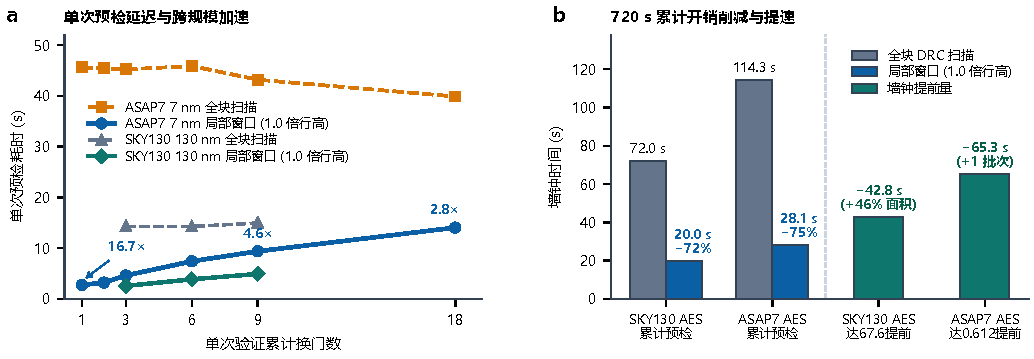
\includegraphics[width=0.94\textwidth]{tcad_20261126/fig5_boxed_drc_scaling_v4_zh.pdf}
\caption{行高自适应$1.0\times H_{\mathrm{row}}$局部窗口化布线前DRC诊断的双工艺加速与端到端收益。（a）130\,nm SKY130HD与7\,nm ASAP7（扩展至18门）单次预检延迟实测缩放曲线；（b）720\,s墙钟内累计预检开销降幅（$-72\%$与$-75\%$）及对应里程碑墙钟提前量。}
\label{fig:boxed_scaling}
\end{figure*}

表~\ref{tab:boxed_drc}与图~\ref{fig:boxed_scaling}(b)汇总了双工艺10臂正反序端到端对照：在SKY130HD AES上，窗口化将单次预检均值由14.40\,s压至3.33\,s（累计开销降72.2\%），使第5批9门端点在正反两序均进入720\,s闭环（回收增46.30\%至98.8448\,\textmu m$^2$）；在7\,nm ASAP7 AES上，单次预检由38.11\,s压至7.03\,s（降75.4\%），达6门端点提前64.7--66.0\,s。

\begin{table*}[t]
\centering
\caption{双工艺10臂正反序$1.0\times H_{\mathrm{row}}$局部窗口化布线前DRC端到端对照（720\,s墙钟预算）}
\label{tab:boxed_drc}
\scriptsize\setlength{\tabcolsep}{3.0pt}
\resizebox{\textwidth}{!}{%
\begin{tabular}{llrrrrrr}
\toprule
\textbf{基准模块（工艺）} & \textbf{策略与诊断模式} & \textbf{完成/派发} & \textbf{窗内合格回收} & \textbf{首达0.01\%} & \textbf{共同大目标首达} & \textbf{单次/累计} & \textbf{正反序一致性} \\
 & & \textbf{（正/反序）} & \textbf{/\textmu m$^2$（池捕获\%）} & \textbf{正/反序 (s)} & \textbf{正/反序 (s)} & \textbf{预检均值 (s)} & \textbf{与复修} \\
\midrule
\multirow{2}{*}{SKY130HD AES}
 & 全块诊断FAECO & 4/5 · 4/5 & 67.5648（34.18\%） & 478.99 / 490.16 & 614.89 / 626.91\textsuperscript{a} & 14.40 / 71.96 & 一致 · 0复修 \\
 & \textbf{窗口化FAECO（$1.0H_{\mathrm{row}}$）} & \textbf{5/6 · 5/6} & \textbf{98.8448（50.00\%）} & \textbf{451.41 / 448.89} & \textbf{580.84 / 575.38}\textsuperscript{a} & \textbf{3.33 / 19.98} & \textbf{一致 · 0复修} \\
\midrule
\multirow{3}{*}{ASAP7 AES}
 & 窗口化灵敏度单门（$1.0H_{\mathrm{row}}$） & 3/4 · 3/4 & 0.30618（17.36\%） & 500.72 / 495.67 & 未达标\textsuperscript{b} & 3.71 / 14.82 & 一致 · 0复修 \\
 & 全块诊断FAECO & 2/3 · 2/3 & 0.61236（34.71\%） & 367.99 / 368.67 & 575.08 / 575.74\textsuperscript{b} & 38.11 / 114.34 & 一致 · 0复修 \\
 & \textbf{窗口化FAECO（$1.0H_{\mathrm{row}}$）} & \textbf{3/4 · 3/4} & \textbf{0.61236（34.71\%）} & \textbf{331.44 / 332.95} & \textbf{510.36 / 509.78}\textsuperscript{b} & \textbf{7.03 / 28.10} & \textbf{一致 · 0复修} \\
\bottomrule
\end{tabular}%
}

\vspace{2pt}
\parbox{\textwidth}{\footnotesize \textsuperscript{a}SKY130HD AES共同大目标为67.5648\,\textmu m$^2$（6门）；窗口化FAECO在714.54/706.87\,s于正反两序均验收9门98.8448\,\textmu m$^2$。\textsuperscript{b}ASAP7 AES共同大目标为0.61236\,\textmu m$^2$（6门）；全部10臂独立全块终检DRC=0、天线=0，SEC均全证。}
\end{table*}

\paragraph{RCX/STA重复确定性与保持时间容差$\varepsilon_h$敏感性}
针对式~\eqref{eq:obj}中$\varepsilon_h=0.001$\,ps（1\,fs）的数值可靠性，我们在SKY130HD AES与ASAP7 UART的同一冻结版图上各独立重复执行3次完整OpenRCX提取与三工艺角OpenSTA分析：两基准3次提取的去日期SPEF哈希逐字节一致，FF/TT/SS Setup/Hold读数极差严格为$0.000$\,ps，证实当前工具链下1\,fs容差不受随机数值抖动影响。进一步在全部主实验已记录物理试探日志上统计$\varepsilon_h\in\{0.001, 0.01, 0.1, 1.0\}$\,ps的离线敏感性：SKY130HD AES窗口矩阵中8/19次试探在0.001与0.01\,ps下均被Hold拒收（最差$-0.158$\,ps），至0.1\,ps降为4/19；ASAP7 UART上136次试探中Hold拒收数随容差由64（0.001\,ps）依次降至48（0.01\,ps）、18（0.1\,ps）与0（1.0\,ps，最差$-0.180$\,ps）；ASAP7 AES窗口矩阵仅2/16次试探在0.001\,ps下因$-0.0022$\,ps微幅退化被拒（放宽至0.01\,ps即降至0）。可见$\varepsilon_h$作为用户可调护栏，在确定性协议中设定0.001\,ps属最严格保守口径，工业应用可依实际寄生签核不确定度灵活放宽至0.01--0.1\,ps。

\subsection{绝对时序收敛基准、参数敏感性与扩展电路验证}
\label{sec:tc_sens}

\paragraph{绝对时序收敛（Timing-closed）基准实测}
为检验FAECO在三工艺角Setup/Hold均已绝对收敛（无残留负松弛）的工业场景下的有效性，在ASAP7 UART-TC（500\,ps周期，FF/TT/SS初始Setup WNS依次为$+255.85$、$+190.42$、$+30.29$\,ps，Hold WNS依次为$+50.31$、$+67.50$、$+54.05$\,ps，1\%预算5.0\,ps）上运行同一$1.0\times H_{\mathrm{row}}$窗口后端720\,s对照（表~\ref{tab:tc_sens}上部）。FAECO交付0.83106\,\textmu m$^2$（13/18门，功能单元面积降1.052\%，时间平均收益0.456\,\textmu m$^2$，去重命中2次），相对窗口单门（0.68526\,\textmu m$^2$，0.363\,\textmu m$^2$）提升21.3\%面积与25.6\%时间平均收益，相对窗口固定微批次（0.33534\,\textmu m$^2$，0.240\,\textmu m$^2$）取得2.48倍面积与1.90倍时间平均收益；且交付版图三工艺角Setup/Hold仍全部严格非负（保持\textbf{Timing-closed}状态，0\,DRC，SEC全证）。

\paragraph{微批次宽度$b$与候选池规模$K$参数敏感性}
在ASAP7 UART同一$1.0\times H_{\mathrm{row}}$窗口后端与720\,s预算下，系统扫描$b\in\{1,2,3,6,9,18\}$（固定$K=18$）及$K\in\{9,18,36\}$（固定$b=3$，其中$K=36$由全网表独立枚举36个互异实例，静态上界2.72646\,\textmu m$^2$），结果汇总于表~\ref{tab:tc_sens}下部与图~\ref{fig:ablation}(c)：（1）随批宽$b$增大，终态合格面积与时间平均收益呈典型倒U形态——$b=1$缺乏批摊销与暂缓重排（0.68526\,\textmu m$^2$，AUC 0.372），\textbf{$b\in\{2,3\}$达到性能峰值}（0.83106\,\textmu m$^2$，AUC 0.526与0.491），而$b\ge 6$因大批次频繁触发Hold拒收与深层二分（如$b=6$去重命中6次、评估21次）导致有效收益回落至0.685--0.744\,\textmu m$^2$（AUC降至0.285--0.335），实证了默认$b=3$的合理性；（2）扩展候选池规模时，合格面积由$K=9$的0.49572\,\textmu m$^2$（0.627\%）持续攀升至$K=18$的0.83106\,\textmu m$^2$（1.052\%）及\textbf{$K=36$的1.50174\,\textmu m$^2$（19/36门，功能单元面积降1.901\%，AUC达0.722\,\textmu m$^2$）}，证实主实验统一的$K=18$仅作为跨设计公平基准下限，而非FAECO的可回收上限。

\begin{table}[t]
\centering
\caption{绝对时序收敛基准实测（ASAP7 UART-TC）与$b$/$K$参数敏感性（720\,s，$1.0H_{\mathrm{row}}$窗口后端）}
\label{tab:tc_sens}
\scriptsize\setlength{\tabcolsep}{2.4pt}
\resizebox{\columnwidth}{!}{%
\begin{tabular}{llrrrrr}
\toprule
\textbf{实验组} & \textbf{配置} & \textbf{合格面积/\textmu m$^2$} & \textbf{功能/池\%} & \textbf{时间平均} & \textbf{评估} & \textbf{去重} \\
 & & \textbf{（合格门数）} & & \textbf{收益/\textmu m$^2$} & \textbf{次数} & \textbf{命中} \\
\midrule
\multirow{3}{*}{\shortstack[l]{Timing-closed\\(500\,ps)}}
 & 窗口单门 & 0.68526（11） & 0.867 / 58.0 & 0.363 & 18 & 0 \\
 & 窗口固定批 & 0.33534（6） & 0.424 / 28.4 & 0.240 & 6 & 0 \\
 & \textbf{窗口FAECO} & \textbf{0.83106（13）} & \textbf{1.052 / 70.4} & \textbf{0.456} & \textbf{18} & \textbf{2} \\
\midrule
\multirow{6}{*}{\shortstack[l]{批宽敏感性\\($K=18$)}}
 & $b=1$ & 0.68526（11） & 0.867 / 58.0 & 0.372 & 18 & 0 \\
 & \textbf{$b=2$} & \textbf{0.83106（13）} & \textbf{1.052 / 70.4} & \textbf{0.526} & \textbf{16} & \textbf{1} \\
 & \textbf{$b=3$（默认）} & \textbf{0.83106（13）} & \textbf{1.052 / 70.4} & \textbf{0.491} & \textbf{18} & \textbf{2} \\
 & $b=6$ & 0.72900（11） & 0.923 / 61.7 & 0.302 & 21 & 6 \\
 & $b=9$ & 0.68526（11） & 0.867 / 58.0 & 0.285 & 20 & 2 \\
 & $b=18$ & 0.74358（12） & 0.941 / 63.0 & 0.335 & 20 & 3 \\
\midrule
\multirow{3}{*}{\shortstack[l]{池规模敏感性\\($b=3$)}}
 & $K=9$ & 0.49572（7） & 0.627 / 73.9 & 0.341 & 8 & 1 \\
 & $K=18$（默认） & 0.83106（13） & 1.052 / 70.4 & 0.491 & 18 & 2 \\
 & \textbf{$K=36$} & \textbf{1.50174（19）} & \textbf{1.901 / 55.1} & \textbf{0.722} & \textbf{23} & \textbf{1} \\
\bottomrule
\end{tabular}%
}
\end{table}

\paragraph{多预算事后筛选、选择性回退与十电路扩展验证}
为补充更广谱电路族上的行为观察，本节另以固定评估次数上限（6--10次重布线）与名义典型角$B_W=10$\,ps口径汇总23个ISCAS89/ITC-99电路的扩展验证（与前述720\,s多角协议分开报告）。在SKY130 \texttt{s382}既有52个物理实测端点池上的事后筛选显示（表~\ref{tab:budget_pool}，注：该表反映不同预算下既有实测池的合格集扩张，而非独立在线重跑轨迹）：零预算下仅6个端点合格（功能单元面积降0.59\%，$\Delta\text{WNS}=+1.71$\,ps），放宽至5--10\,ps后以3.10\,ps建立时间微幅让渡换取Resizer净新增面积28.91\%回收（功能单元面积降4.40\%，Hold改善3.58\,ps）。跨8个ISCAS89与15个ITC-99电路的固定寄生选择性回退分别安全回退61\%（65/107）与88.3\%（857/971）的冗余放大；在含359处修改的\texttt{b22}上，转折门前缀二分仅10次STA即定位单一临界异或门并回退356处修改。

在十个SKY130基准（\texttt{s382}--\texttt{s953}、\texttt{b04}、\texttt{b05}、\texttt{b11}、\texttt{b12}）的独立物理闭环对照中（表~\ref{tab:ten_circuits}，十电路均值均将零收益电路按0.00\%计入）：原生回收与离线五轮LR均未交付合格解；固定寄生灵敏度批处理仅5/10有效；在线单门贪心9/10有效且平均面积降幅略高（2.11\%，但于\texttt{s953}上为0.00\%）；FAECO实现10/10全有效（平均面积降幅2.01\%，总/组合功耗均降0.96\%/3.72\%），以0.10个百分点的均值微小折让换取100\%跨电路稳健性，并在规模最大的\texttt{b12}上实现单门2.0倍回收（0.82\%对0.41\%）。在5,494实例的\texttt{b15}上，局部增量绕线6轮均在185--201\,s达成零DRC（全片重布1,426\,s仍留66处DRC），回收0.26\%面积并降静态漏电0.84\%。

\begin{table}[t]
\centering
\caption{SKY130 \texttt{s382}既有52物理端点池的四档预算事后筛选}
\label{tab:budget_pool}
\scriptsize\setlength{\tabcolsep}{3.0pt}
\resizebox{\columnwidth}{!}{%
\begin{tabular}{lrrrr}
\toprule
\textbf{建立时间预算} & \textbf{合格端点数} & \textbf{功能面积降幅} & \textbf{净增回收} & \textbf{$\Delta$WNS / Hold (ps)} \\
\midrule
0\,ps（严格） & 6 & 0.59\% & 3.91\% & $+$1.71 / $+$0.00 \\
5\,ps & 15 & 4.40\% & 28.91\% & $-$3.10 / $+$3.58 \\
10\,ps & 19 & 4.40\% & 28.91\% & $-$3.10 / $+$3.58 \\
20\,ps & 21 & 4.40\% & 28.91\% & $-$3.10 / $+$3.58 \\
\bottomrule
\end{tabular}%
}
\end{table}

\begin{table}[t]
\centering
\caption{十个SKY130基准五方法独立物理闭环汇总（$B_W=10$\,ps，6--10次评估，零收益按0计入均值）}
\label{tab:ten_circuits}
\scriptsize\setlength{\tabcolsep}{2.6pt}
\resizebox{\columnwidth}{!}{%
\begin{tabular}{lrrrr}
\toprule
\textbf{对比方法} & \textbf{有效电路} & \textbf{平均面积降幅} & \textbf{总/组合功耗均降} & \textbf{物理与等价验证} \\
\midrule
OpenROAD原生回收 & 0 / 10 & 0.00\% & --- & 零触发 \\
离线五轮冻结寄生LR & 0 / 10 & 0.00\% & --- & 10/10超预算 \\
冻结寄生灵敏度批处理 & 5 / 10 & 0.14\% & --- & 5/10通过 \\
灵敏度在线单门贪心 & 9 / 10 & \textbf{2.11\%} & --- & 9/10（\texttt{s953}为0\%） \\
\textbf{FAECO独立闭环} & \textbf{10 / 10} & 2.01\% & \textbf{$-$0.96\% / $-$3.72\%} & \textbf{10/10全通过} \\
\bottomrule
\end{tabular}%
}
\end{table}

% ============================================================
% §6 讨论与适用边界
% ============================================================
\section{讨论与适用边界}

综合理论分析与双工艺实证，本文归纳所提机制的作用边界与工程启示：
\begin{enumerate}
\item \textbf{物理使能后端与启发式搜索前端的分工定位。} 本文最核心的技术贡献在于以行高自适应局部窗口DRC诊断与保护式局部重布线作为布线后跨占位ECO的物理使能机制；而在搜索层面上，FAECO是面向跨设计稳健性的限时启发式策略，而非对单个任意设计具备全局最优保证的数学求解器。Hybrid FAECO通过引入有界乐观全池探针有效融合了大批次高吞吐与微批次跨设计稳健性，并在实证中呈现出清晰的早窗时间平均收益与终态回收面积权衡。
\item \textbf{局部窗口诊断的几何、规则与规模边界。} 命题~1的覆盖完备性严格限定于引脚层局部短路与成对间距规则；最小面积规则及详细重布线期间由新走线动态生成的次生违例（如在SKY130HD \texttt{gcd}固定三门测试中观察到的3处重布后底层短路）须由终检全块DRC与单次定向复修保障。此外，7\,nm扩展测试表明窗口化诊断在万门级模块上具有显著加速（最高16.69倍），而在不足千网的微型模块上收益有限，实际部署可按版图规模自动切换。
\item \textbf{多角验证边界与工艺/基准局限。} 本文实验在FF/TT/SS三工艺角加载对应标准单元库并共享单次提取名义SPEF，尚未引入独立RC角寄生提取与商业签核工具；主实验四个开源参考起点包含残留建立时间负松弛，虽已通过新增绝对时序收敛基准（ASAP7 UART-TC）补强验证，但更大规模工业级Timing-closed多时钟域SoC宏模块与多档独立预算在线轨迹仍属后续研究重点。当网表常规逻辑已映射至最小驱动档（如\texttt{b14}）时，纯降尺寸空间趋于枯竭，需结合等价逻辑重构以拓展上界。
\end{enumerate}

% ============================================================
% §7 结论
% ============================================================
\section{结论}

本文面向有限时间预算下的布线后门级面积与功耗回收问题，提出了以局部冲突诊断与保护式重布线为核心的ECO框架FAECO。通过建立区分ECO合格与绝对时序收敛的多角物理验证模型、推导并依双工艺真实技术LEF规则核验行高自适应$1.0\times H_{\mathrm{row}}$局部窗口化布线前DRC诊断的几何覆盖边界（命题~1），以及设计耦合有界乐观全池探针与保持时间反馈自适应微批次的混合调度机制（Hybrid FAECO），在130\,nm SKY130HD与7\,nm ASAP7双工艺基准上取得了系统验证。实验表明：局部窗口诊断在37组历史回放中与全块DRC的56处非零违例标记完全匹配（未观察到漏报）并实现3.04--16.69倍单次加速；受控消融证实精确锁定冲突邻网可同时消除冗余重布与亚皮秒保持时间退化，同一窗口后端下直连电容代理重排在SKY130HD AES上独立贡献2.93倍终态面积增益（98.8448\,\textmu m$^2$），Hybrid FAECO进一步在251\,s内兑现100\%候选池收益（197.6896\,\textmu m$^2$），并在其余三主基准及绝对时序收敛7\,nm基准上保持100\%稳健交付与提取寄生功耗同步下降。

\vspace{0.22cm}
\noindent\textbf{致谢。}
感谢OpenROAD、OpenSTA与Yosys开源社区提供的数字物理实现与形式验证工具链。

% ============================================================
% 参考文献
% ============================================================
\begingroup\footnotesize\linespread{0.88}\selectfont\setlength{\parskip}{0pt}
\interlinepenalty=10000
\begin{thebibliography}{30}
\setlength{\itemsep}{0pt}\setlength{\parsep}{0pt}

\bibitem{chinnery2002closing}
Chinnery D, Keutzer K. Closing the gap between ASIC and custom: Tools and techniques for high-performance ASIC design[M]. Boston: Kluwer Academic Publishers, 2002.

\bibitem{openroad}
Ajayi T, Chhabria V A, Foga\c{c}a M, et al. Toward an open-source digital flow: First learnings from the OpenROAD project[C]//Proceedings of the 56th ACM/IEEE Design Automation Conference (DAC). 2019: 1--4.

\bibitem{lee2012eco}
Lee J, Gupta P. ECO cost measurement and incremental gate sizing for late process changes[J]. ACM Transactions on Embedded Computing Systems (TECS), 2012, 9(4): Article 39.

\bibitem{fatemi2019sizer}
Fatemi H, Kahng A B, Lee H, et al. Enhancing sensitivity-based power reduction for an industry IC design context[J]. Integration, the VLSI Journal, 2019, 66: 96--111.

\bibitem{cheng2023dagsizer}
Cheng C K, Holtz C, Kahng A B, et al. DAGSizer: A directed graph convolutional network approach to discrete gate sizing of VLSI graphs[J]. ACM Transactions on Design Automation of Electronic Systems (TODAES), 2023, 28(4): Article 52.

\bibitem{tritonroutewxl}
Kahng A B, Wang L, Xu B. TritonRoute-WXL: The open source router with integrated DRC engine[J]. IEEE Transactions on Computer-Aided Design of Integrated Circuits and Systems, 2022, 41(4): 1076--1089.

\bibitem{yosys}
Wolf C. \textit{Yosys Open SYnthesis Suite}[EB/OL]. 2026. \url{https://github.com/YosysHQ/yosys}

\bibitem{ozdal2012ispd}
Ozdal M M, Burns S M, Hu J. Gate sizing and device technology selection algorithms for high-performance industrial designs[C]//Proceedings of the IEEE/ACM International Conference on Computer-Aided Design (ICCAD). 2011: 724--731.

\bibitem{hu2013ispd}
ACM International Symposium on Physical Design. ISPD 2013 discrete gate sizing contest and benchmark suite[EB/OL]. 2013. \url{https://www.ispd.cc/contests/13/ispd2013_contest.html}

\bibitem{chen1999fast}
Chen C P, Chu C C N, Wong D F. Fast and exact simultaneous gate and wire sizing by Lagrangian relaxation[J]. IEEE Transactions on Computer-Aided Design of Integrated Circuits and Systems, 1999, 18(7): 1014--1025.

\bibitem{flach2014effective}
Flach G, Reimann T, Posser G, et al. Effective method for simultaneous gate sizing and $V_{th}$ assignment using Lagrangian relaxation[J]. IEEE Transactions on Computer-Aided Design of Integrated Circuits and Systems, 2014, 33(4): 546--557.

\bibitem{timing_budget}
Mangiras D, Chinnery D G, Dimitrakopoulos G. Task-based parallel programming for gate sizing[J]. IEEE Transactions on Computer-Aided Design of Integrated Circuits and Systems, 2023, 42(4): 1309--1322.

\bibitem{trident2}
Kahng A B, Kang S, Lee H, et al. High-performance gate sizing with a signoff timer[C]//Proceedings of the IEEE/ACM International Conference on Computer-Aided Design (ICCAD). 2013: 450--457.

\bibitem{coreeco}
Cheng C K, Kahng A B, Kang I, et al. CoRe-ECO: Concurrent refinement of detailed place-and-route for an efficient ECO automation[C]//IEEE International Conference on Computer Design (ICCD). 2021: 366--373.

\bibitem{sloeco2024}
Jeon J W, Kahng A B, Kang J H, et al. SLO-ECO: Single-line-open aware ECO detailed placement and detailed routing co-optimization[C]//Proceedings of the 25th International Symposium on Quality Electronic Design (ISQED). 2024: 1--8.

\bibitem{openphysyn2020}
Agiza A, Reda S. OpenPhySyn: An open-source physical synthesis optimization toolkit[C]//Proceedings of the Workshop on Open-Source EDA Technology (WOSET). 2020: 1--4.

\bibitem{rlsizer2021}
Lu Y C, Nath S, Khandelwal V, et al. RL-Sizer: VLSI gate sizing for timing optimization using deep reinforcement learning[C]//Proceedings of the 58th ACM/IEEE Design Automation Conference (DAC). 2021: 1--6.

\bibitem{rlccd2023}
Lu Y C, Chan W T, Guo D, et al. RL-CCD: Concurrent clock and data optimization using attention-based self-supervised reinforcement learning[C]//Proceedings of the 60th ACM/IEEE Design Automation Conference (DAC). 2023: 1--6.

\bibitem{pcr2026}
Jiang Z, Pan H, Lan C, Zhu K. Timing-driven logic remapping with local physical context[EB/OL]. arXiv:2610.01918, 2026.

\bibitem{elayout2026}
Fang W, Liang R, Lu Y C, et al. E-Layout: Layout-stage logic restructuring via RL-optimized equality-saturated graph retrieval-augmented generation[EB/OL]. arXiv:2610.26432, 2026.

\bibitem{goalevolve2026}
Liu H, Zhou L, Ren Y, et al. GoalEvolve: From handcrafted algorithm priors to goal-driven evolution of physical design algorithms[EB/OL]. arXiv:2608.16733, 2026.

\bibitem{sta}
OpenSTA Project. \textit{OpenSTA: Gate-level static timing analyzer}[EB/OL]. 2026. \url{https://github.com/The-OpenROAD-Project/OpenSTA}

\end{thebibliography}
\endgroup

\end{document}
